% Author Name: José Areia 
% Author Contact: jose.apareia@gmail.com
% Version: 2.2.10 - 2025-07-18
% Public Repository: https://github.com/joseareia/ipleiria-thesis
% Wiki/Getting Help: https://github.com/joseareia/ipleiria-thesis/wiki

%%% Document Options %%%
\documentclass[
    language=french,
    school=eniad,
    docstage=final,
    media=paper,
    bookprint=false,
    linkcolor=red!45!black,
    chapterstyle=classic,
    coverstyle=classic,
    aiack=true
]{IPLeiriaThesis} % Refer to the Wiki for a list of available options.

%%% Document Version %%%
\DocumentVersion{1.0.0} % Required only if the 'docstage' is set to 'working'.

%%% Document Metadata %%%
% First Author (Mandatory)
\FirstAuthor{AbdElMalek Lamkadem}
% \FirstAuthorNumber{2230455}

% Second Author (Optional)
\SecondAuthor{Jane Smith}
% \SecondAuthorNumber{2230456}

% Third Author (Optional)
\ThirdAuthor{July Smith}
% \ThirdAuthorNumber{2230457}

% Supervisor (Mandatory)
\Supervisor{John Smith}
\SupervisorMail{joe.smith@ipleiria.pt}
% Please provide: [Current Title, Affiliation]
\SupervisorTitle{Full Professor, Polytechnic of Leiria} 

% Co-Supervisor (Optional)
% \CoSupervisor{Steve Smith}
% \CoSupervisorMail{steve.smith@ipleiria.pt}
% \CoSupervisorTitle{Associate Professor, Polytechnic of Leiria}

% Second Co-Supervisor (Optional)
% \SecCoSupervisor{Shak Smith}
% \SecCoSupervisorMail{shak.smith@ipleiria.pt}
% \SecCoSupervisorTitle{Associate Researcher, Computer Science \& Communication Research Centre}

% Title (Mandatory)
\Title{rapport de stage pfa a majal berkane}

% Subtitle (Mandatory)
\Subtitle{developpement de aquadrone une unmanned surface vehicle}

% University (Mandatory)
\University{universitie mohamed premier}

% School (Mandatory)
\School{ecole national de lintelegence artificiel et digital}

% Department (Mandatory)
% \Department{Department of Computer Engineering}

% Degree (Mandatory)
\Degree{robotique \&objects connectes}

% Course (Optional)
% \Course{Offensive \& Defensive Cybersecurity}

% Thesis Theme (Mandatory)
\ThesisType{stage }

% Local & Date (Mandatory)
\Date{Berkane, \DTMmonthname{\month} \number\year}

% Academic Year 
\AcademicYear{2024/25}

%%% Loading of Glossary and Acronyms %%%
\makeglossaries
\loadglsentries{Matter/05-Glossary}
\loadglsentries[\acronymtype]{Matter/06-Acronyms}
\loadglsentries[\symboltype]{Matter/07-Symbols}

\begin{document}

%%% Front Matter %%%
\ifthenelse{\equal{\getLanguage}{portuguese}}{%
    \pdfbookmark[0]{Capa}{capa} % Add entry to PDF bookmarks group.
    \pdfbookmark[1]{Frontispício}{frontispício} % Add entry to PDF.
}{%
    \pdfbookmark[0]{Front Matter}{frontmatter} % Add entry to PDF bookmarks group.
    \pdfbookmark[1]{Cover}{cover} % Add entry to PDF.
}

% Add background picture depending on the 'bwcover' variable.
\ifbwcover
    \newcommand\BackgroundPicCover{%
    \put(0,0){%
    \parbox[b][\paperheight]{\paperwidth}{%
    \vfill
    \centering
    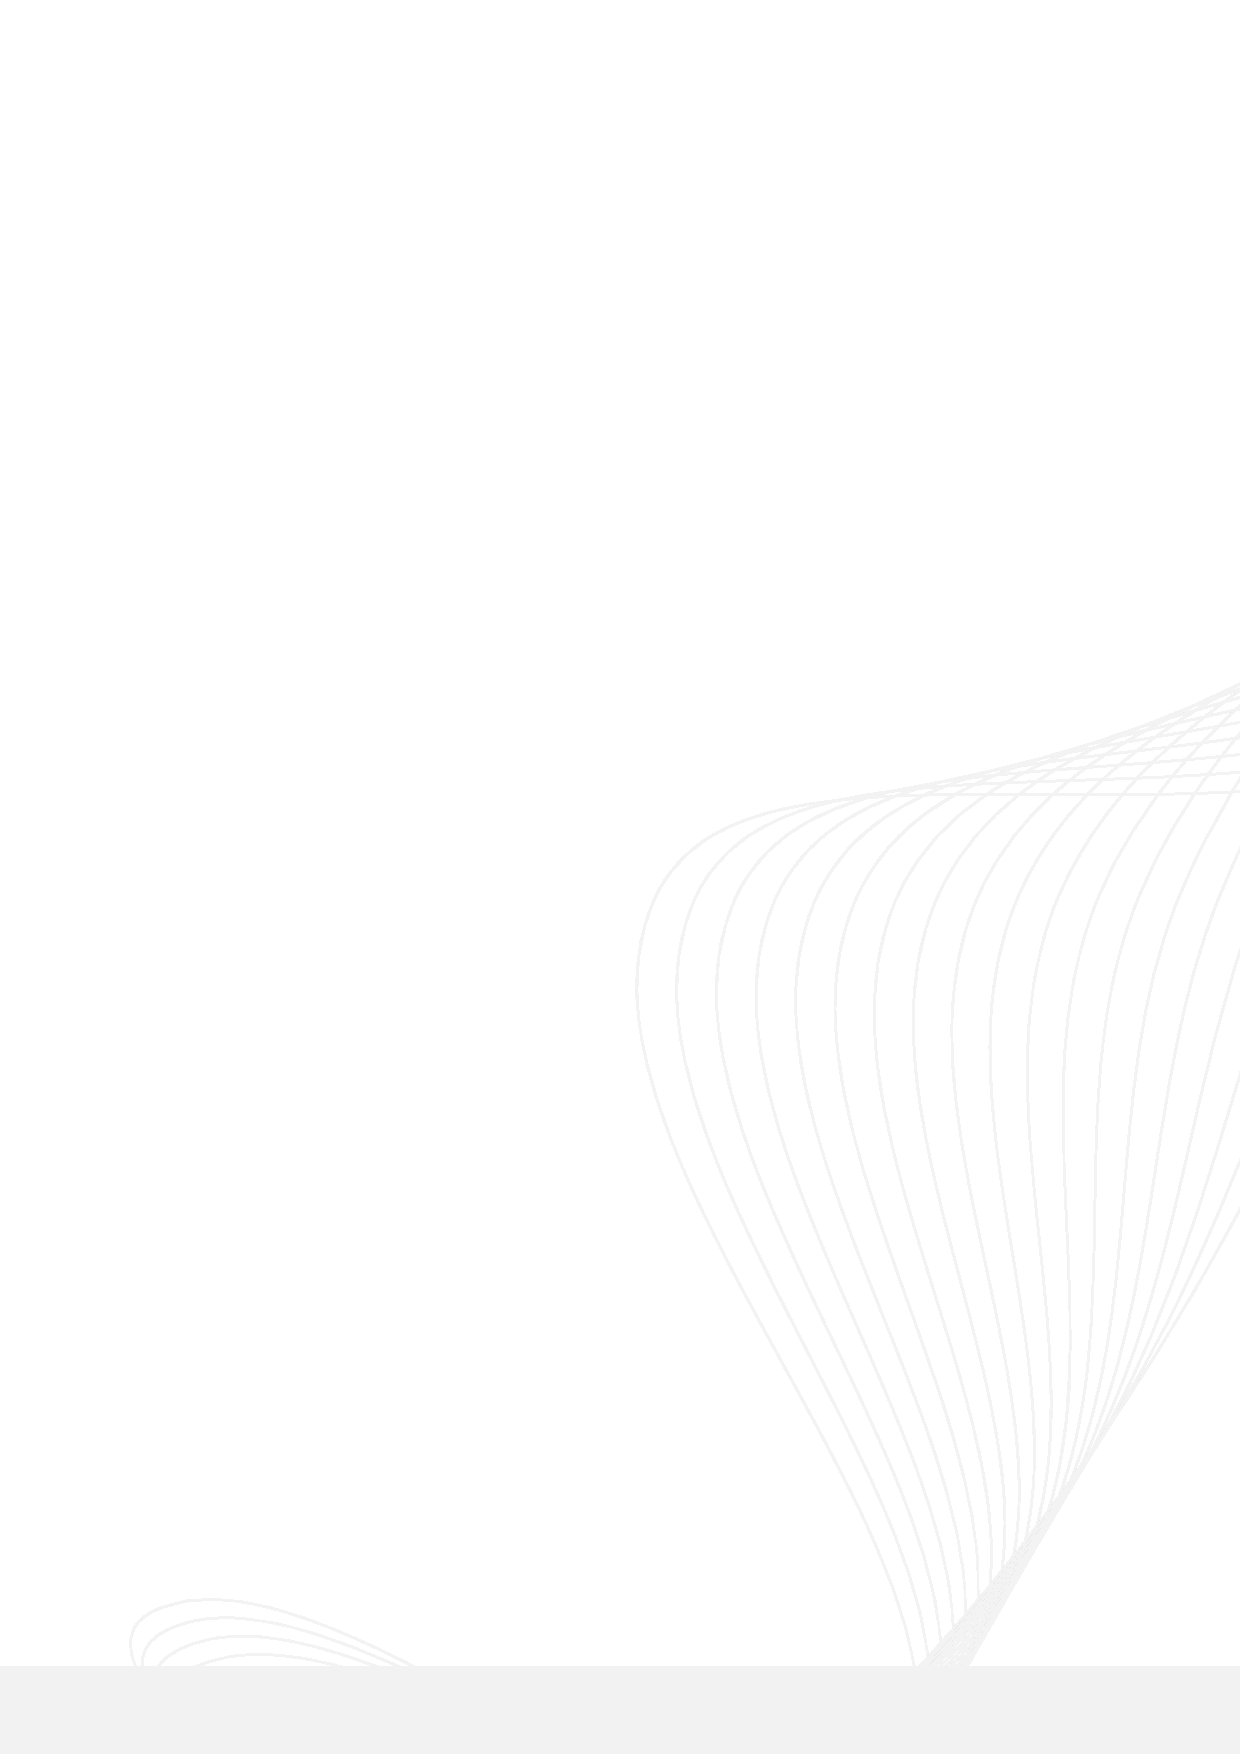
\includegraphics[width=\paperwidth,height=\paperheight,keepaspectratio]{Figures/Theme/Front-Page-BG.pdf}%
    \vfill
    }}}
\else
    \newcommand\BackgroundPicCover{%
    \put(0,0){%
    \parbox[b][\paperheight]{\paperwidth}{%
    \vfill
    \centering
    
\includegraphics[width=\paperwidth,height=\paperheight,keepaspectratio]{Figures/Theme/Cover-BG.pdf}%
    \vfill
    }}}
\fi

\AddToShipoutPictureBG*{\BackgroundPicCover}

\newgeometry{margin=1.98cm, top=2.15cm, bottom=1.47cm}
\begin{titlepage}
    \latofont % Switch to Lato font for the title page.
   
    \ifbwcover
        \color{frontpagedark} % Define the color to use within this page.
    \else
        \color{white} % Define the color to use within this page.
    \fi
    
    \vspace*{\baselineskip} % White space at the top of the page.

    \ifbwcover
        \begin{figure}
            
\includegraphics[width=0.32\linewidth]{Figures/Theme/IPLeiria-Logo-B.pdf}
        \end{figure}
    \else
        \begin{figure}
            
\includegraphics[width=0.32\linewidth]{Figures/Theme/IPLeiria-Logo-W.pdf}
        \end{figure}
    \fi

    \vspace{5.5\baselineskip}

    % Title
	\noindent
    \makebox[\textwidth][l]{%
        \parbox{\dimexpr\textwidth-2.5cm\relax}{
            \setstretch{1.03}
            \raggedright\bfseries\fontsize{20}{26}\selectfont\thetitle
        }
    }

    \vspace{0.8\baselineskip}

    % Subtitle
    \noindent
    \makebox[\textwidth][l]{%
        \parbox{\dimexpr\textwidth-7cm\relax}{
            \setstretch{1.03}
            \raggedright\fontsize{14}{19}\selectfont\subname
        }
    }

    \vspace{35pt}  

    % Author
    {\noindent\bfseries\fontsize{14}{19}\selectfont\firstauthorname}

    \ifdefined\secondauthorname
        \vspace{8pt}
        {\noindent\bfseries\fontsize{14}{19}\selectfont\secondauthorname}
	\fi

    \ifdefined\thirdauthorname
        \vspace{8pt}
        {\noindent\bfseries\fontsize{14}{19}\selectfont\thirdauthorname}
	\fi
 
	\vfill

    % School
	{\noindent\fontsize{10}{12}\selectfont\schoolname}
	
    % Department
	{\noindent\fontsize{10}{12}\selectfont\departmentname}

    % Degree
	{\noindent\fontsize{10}{12}\selectfont\degname}

    % Course
    \ifdefined\coursename
        {\noindent\fontsize{10}{12}\selectfont\coursename}
	\fi

    \vspace{125pt}

    % Local & Date
	{\noindent\fontsize{10}{12}\selectfont\thedate}

    \vspace{68pt}
\end{titlepage}
\restoregeometry\blankpage
\newcommand\BackgroundPicFrontPage{%
    \put(0,0){%
    \parbox[b][\paperheight]{\paperwidth}{%
    \vfill
    \centering
    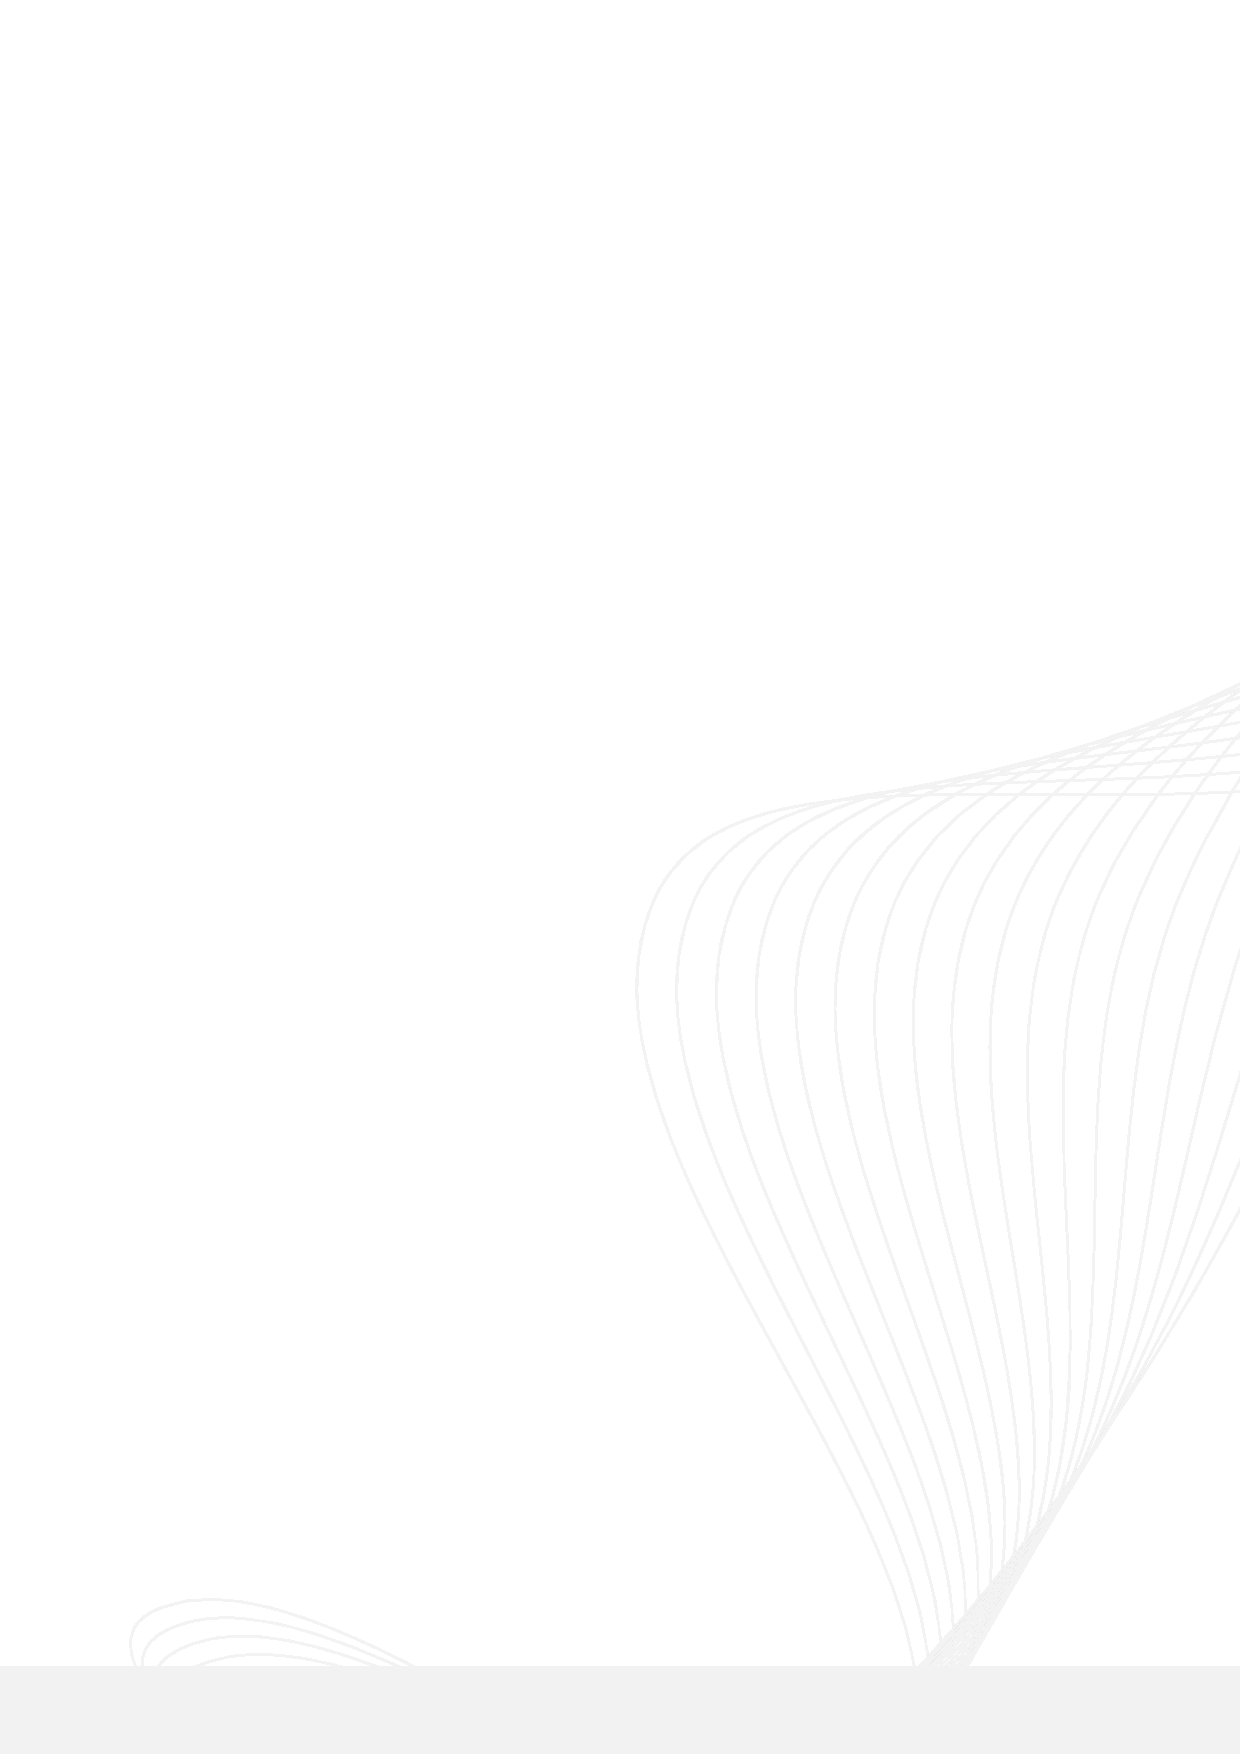
\includegraphics[width=\paperwidth,height=\paperheight,keepaspectratio]{Figures/Theme/Front-Page-BG.pdf}%
    \vfill
}}}
\AddToShipoutPictureBG*{\BackgroundPicFrontPage}

\newgeometry{margin=1.98cm, top=2.15cm, bottom=1.47cm}
\begin{titlepage}
    \latofont
    \color{frontpagedark}
    \vspace*{\baselineskip}

    \ifthenelse{\equal{\SchoolOption}{estg}}{
        \begin{figure}
            
\includegraphics[width=0.485\linewidth]{Figures/Theme/Logotypes/IPLeiria-ESTG-Logo-B.pdf}
        \end{figure}
    }
    
    \ifthenelse{\equal{\SchoolOption}{esad}}{
        \begin{figure}
            
\includegraphics[width=0.485\linewidth]{Figures/Theme/Logotypes/IPLeiria-ESAD-Logo-B.pdf}
        \end{figure}
    }
    
    \ifthenelse{\equal{\SchoolOption}{esslei}}{
        \begin{figure}
            
\includegraphics[width=0.485\linewidth]{Figures/Theme/Logotypes/IPLeiria-ESSLEI-Logo-B.pdf}
        \end{figure}
    }
    
    \ifthenelse{\equal{\SchoolOption}{estm}}{
        \begin{figure}
            
\includegraphics[width=0.485\linewidth]{Figures/Theme/Logotypes/IPLeiria-ESTM-Logo-B.pdf}
        \end{figure}
    }
    
    \ifthenelse{\equal{\SchoolOption}{esecs}}{
        \begin{figure}
            
\includegraphics[width=0.485\linewidth]{Figures/Theme/Logotypes/IPLeiria-ESECS-Logo-B.pdf}
        \end{figure}
    }

    \vspace{3.5\baselineskip}

    % Title.
	\noindent
    \makebox[\textwidth][l]{%
        \parbox{\dimexpr\textwidth-2.5cm\relax}{
            \setstretch{1.03}
            \raggedright\bfseries\fontsize{20}{26}\selectfont\GetTitle
        }
    }

    \vspace{0.8\baselineskip}

    % Subtitle.
    \noindent
    \makebox[\textwidth][l]{%
        \parbox{\dimexpr\textwidth-7cm\relax}{
            \setstretch{1.03}
            \raggedright\fontsize{14}{19}\selectfont\GetSubtitle
        }
    }

    \vspace{35pt}

    % Author.
    {\noindent\bfseries\fontsize{14}{19}\selectfont\GetFirstAuthor}
    
    {\noindent\itshape\fontsize{10}{10}\selectfont Student No. \GetFirstAuthorNumber}

    \ifdefined\GetSecondAuthor
        \vspace{8pt}
        {\noindent\bfseries\fontsize{14}{19}\selectfont\GetSecondAuthor}
	\fi

    \ifdefined\GetThirdAuthor
        \vspace{8pt}
        {\noindent\bfseries\fontsize{14}{19}\selectfont\GetThirdAuthor}
	\fi

    \vspace{58pt}    

    {
    \noindent
    \latofont
    \fontsize{10}{12}\selectfont
    \renewcommand{\arraystretch}{0.1}
    \hspace*{-2.5pt}\begin{tabular}{@{}r@{\hspace{5pt}}>{\raggedright\arraybackslash}m{6cm}@{}}
        \textbf{Supervisor:} & \GetSupervisor \\ [-.7ex]
        & \setstretch{0.9}{\fontsize{8}{10}\selectfont\itshape \GetSupervisorTitle} \\ [2ex]
        
        \ifdefined\GetCoSupervisor
            \textbf{Co-supervisor:} & \GetCoSupervisor \\ [-.7ex]
            & \setstretch{0.9}{\fontsize{8}{10}\selectfont\itshape \GetCoSupervisorTitle} \\ [.5ex]
        \fi

        \ifdefined\GetSecCoSupervisor        
            & \GetSecCoSupervisor \\ [-.7ex]
            & \setstretch{0.9}{\fontsize{8}{10}\selectfont\itshape \GetSecCoSupervisorTitle} \\
        \fi
    \end{tabular}
    }
    
    \vfill
	
    % School.
	{\noindent\fontsize{10}{12}\selectfont\GetSchool}
	
    % Department.
	{\noindent\fontsize{10}{12}\selectfont\GetDepartment}

    % Degree.
	{\noindent\fontsize{10}{12}\selectfont\GetDegree}

    % Course.
    \ifdefined\GetCourse
        {\noindent\fontsize{10}{12}\selectfont\GetCourse}
	\fi

    \vspace{45pt}

    % Thesis option.
	{\noindent\fontsize{10}{12}\itshape\selectfont\GetThesisType}

    \vspace{45pt}

    % Local and date.
	{\noindent\fontsize{10}{12}\selectfont\GetDate}

    \vspace{68pt}
\end{titlepage}
\restoregeometry
\MediaOptionLogicBlank

%%% Copyright Statement %%%
% \pagenumbering{gobble} % Prevent page numbering.

\vspace*{\fill}

\ifthenelse{\equal{\LanguageOption}{portuguese}}{%
    \noindent \textbf{\GetTitle}
    
    \noindent Copyright \textcopyright~\the\year{} - \GetFirstAuthor, \GetSchool.
    
    \vspace{.575em}
    
    \noindent A presente dissertação é um trabalho original, elaborado exclusivamente para este fim, tendo sido devidamente citados todos os autores cujos estudos e publicações contribuíram para a sua elaboração. É permitida a sua reprodução parcial com indicação do autor e referência ao grau, ano letivo, instituição - \textit{Politécnico de Leiria} - e data da defesa pública.
}{%
    \noindent \textbf{\GetTitle}
    
    \noindent Copyright \textcopyright~\the\year{} - \GetFirstAuthor, \GetSchool.
    
    \vspace{.575em}
    
    \noindent This dissertation is original work, written solely for this purpose, and all the authors whose studies and publications contributed to it have been duly cited. Partial reproduction is allowed with acknowledgment of the author and reference to the degree, academic year, institution - \textit{Polytechnic University of Leiria} - and public defense date.
}

\vspace*{\fill}

\plainblankpage

%%% Roman Numeration %%%
\pagenumbering{roman}

%%% Acknowledgements %%%
\ifthenelse{\equal{\LanguageOption}{portuguese}}{%
    \chapter*{Agradecimentos}
}{%
    \chapter*{Acknowledgements}
}

In the \textit{Acknowledgment} section, express your gratitude to those who helped and supported your work. Start by thanking your advisors, mentors, or supervisors who provided guidance and expertise. Mention any colleagues, classmates, or team members who contributed to discussions or offered assistance. You can also acknowledge specific organisations, institutions, or funding sources that supported your research or work. Lastly, include any personal acknowledgments for family or friends who offered encouragement and moral support during the project. Keep this section sincere, concise, and professional.

\plainblankpage

%%% Abstract %%%
\thispagestyle{plain}


% English Abstract 
\pdfbookmark[1]{Abstract}{abstract}
\chapter*{Abstract}
\guideinfo{In the \textit{Abstract} section, provide a concise summary of your project, highlighting the key points. Begin with a brief statement of the problem or objective, followed by a description of your approach or methodology. Summarise the main results or findings, emphasising their significance or implications. Conclude with a sentence or two on the overall contribution or impact of your work. Keep the abstract clear and focused, ideally within 150-250 words, to give readers a quick understanding of your research and its importance.}
\keywordsen{Keyword A, Keyword B, Keyword C.}
\MediaOptionLogicBlank

% French Abstract 
\pdfbookmark[1]{Résumé}{resume}
\chapter*{Résumé}
\guideinfo{Dans la section \textit{Résumé}, présentez un résumé concis de votre projet en mettant en avant les points clés. Commencez par une brève déclaration du problème ou de l'objectif, suivie d'une description de votre approche ou méthodologie. Résumez les principaux résultats ou conclusions en soulignant leur importance ou leurs implications. Concluez par une ou deux phrases sur la contribution globale ou l'impact de votre travail. Le résumé doit être clair et concis (idéalement 150-250 mots) pour permettre aux lecteurs de comprendre rapidement votre travail et son importance.}
\keywordsen{Mot-clé A, Mot-clé B, Mot-clé C.}
\MediaOptionLogicBlank

% Arabic Abstract 
% \pdfbookmark[1]{ملخص}{abstract-ar}
% \chapter*{ملخص}
% \guideinfo{في قسم \textit{الملخص}، قدّم ملخصًا موجزًا لمشروعك مع إبراز النقاط الرئيسية. ابدأ ببيان مختصر للمشكلة أو الهدف، يليه وصف لمنهجيتك أو طريقة بحثك. لخّص النتائج أو الاستنتاجات الرئيسية مع التأكيد على أهميتها أو تداعياتها. اختتم بجملة أو جملتين حول الإسهام العام أو تأثير عملك. يجب أن يكون الملخص واضحًا وموجزًا (150-250 كلمة مثاليًا) لتمكين القراء من فهم عملك وأهميته بسرعة.}
% \keywordspt{كلمة مفتاحية أ، كلمة مفتاحية ب، كلمة مفتاحية ج.}
% \MediaOptionLogicBlank

%%% AI Acknowledgement %%%
\ifthenelse{\equal{\AiAckOption}{true}}{%
    \ifthenelse{\equal{\LanguageOption}{portuguese}}{%
        \chapter*{Declaração sobre o Uso de Inteligência Artificial}

        \guideinfo{É uma boa prática académica indicar brevemente como, porquê e quando a IA foi utilizada. Explicar as ações tomadas e as razões que lhes estão subjacentes promove a reflexão crítica, aprofunda a compreensão do papel da IA na aprendizagem e ajuda a avaliar o seu impacto na qualidade e integridade do trabalho. Esta página pode ser removida definindo a opção \texttt{aiack} como \texttt{false} nas opções da classe do documento.}
    
        \vspace{2em}
        
        \exampleinfo{%
        Reconheço a utilização do ChatGPT (\url{https://chatgpt.com}) para aperfeiçoar o tom académico e melhorar a precisão linguística deste trabalho, incluindo aspectos de gramática, pontuação e vocabulário.
        
        \vspace{1em}
        
        \noindent\textbf{Descrição da Utilização}
        
        \prompt[1]{Num parágrafo, descreva simplesmente o que é o LaTeX.}
        
        \aioutput[1]{O LaTeX é um sistema de composição de alta qualidade, normalmente utilizado para produzir documentos científicos e matemáticos, devido ao seu poderoso manuseamento de fórmulas e bibliografias. Ao contrário dos processadores de texto, utiliza ficheiros de texto simples com etiquetas de marcação para definir a estrutura e a formatação de um documento, permitindo um controlo preciso da disposição e do aspeto. É especialmente popular no meio académico e na investigação para a criação de teses, artigos de revistas e apresentações.}
        }
    }{%
        \chapter*{AI Acknowledgement}

        \guideinfo{It is good academic practice to briefly state how, why, and when AI was used. Explaining both the actions taken and the reasons behind them encourages critical reflection, deepens understanding of AI's role in learning, and supports the evaluation of its impact on your work’s quality and integrity. This page can be removed by setting the option \texttt{aiack} to \texttt{false} in the document class options.}

        \vspace{2em}
        
        \exampleinfo{%
        I acknowledge the use of ChatGPT (\url{https://chatgpt.com}) to refine the academic tone and improve the linguistic accuracy of this work, including aspects of grammar, punctuation, and vocabulary.
        
        \vspace{1em}
        
        \noindent\textbf{Description of Use}
        
        \prompt[1]{In a paragraph, simply describe what LaTeX is.}
        
        \aioutput[1]{LaTeX is a high-quality typesetting system commonly used for producing scientific and mathematical documents due to its powerful handling of formulas and bibliographies. Unlike word processors, it uses plain text files with markup tags to define the structure and formatting of a document, allowing precise control over layout and appearance. It is especially popular in academia and research for creating theses, journal articles, and presentations.}
        }
    }
    
    \MediaOptionLogicBlank   
}{}

%%% Table of Contents, List of Figures and List of Tables %%%
\bookmarktocentry\tableofcontents
\listoffigures
\listoftables

%%% Print: Glossary and Acronyms %%%
\glossarytoc\printnormalglossary
\acronymtoc\printacronymglossary
\symboltoc\printsymbolglossary

%%% Arabic Numeration %%%
\pagenumbering{arabic}

%%% Chapters (**Insert Yours Here**) %%%
\chapter[Introduction générale]{Introduction générale}
\label{cp:introduction-generale}

{
\parindent0pt

\section{Contexte du projet et importance dans le domaine maritime}
Le domaine maritime représente un enjeu crucial pour l'économie mondiale, la sécurité et la préservation de l'environnement. La surveillance des océans, la gestion des ressources halieutiques et la protection des écosystèmes marins nécessitent des solutions innovantes et adaptées aux défis spécifiques de l'environnement marin.

Les technologies autonomes et la robotique maritime émergent comme des solutions prometteuses pour répondre à ces défis. Les véhicules de surface sans équipage (USV - Unmanned Surface Vehicles) offrent de nouvelles possibilités pour la surveillance maritime, la collecte de données océanographiques et l'assistance à la pêche, tout en réduisant les risques pour les équipages humains.

\begin{block}[note]
Cette introduction présente le cadre général du projet AquaDrone, un véhicule autonome multifonction développé pour répondre aux défis spécifiques de l'environnement maritime marocain et méditerranéen.
\end{block}

\section{Problématique générale}
Malgré les avancées technologiques récentes, les systèmes nautiques actuels présentent plusieurs limitations qui freinent leur adoption généralisée et leur efficacité opérationnelle. Les défis incluent la robustesse face aux conditions marines difficiles, l'autonomie énergétique limitée, la fiabilité des communications en mer et l'intégration harmonieuse de multiples capteurs et systèmes.

La complexité de l'environnement maritime - caractérisé par des conditions météorologiques variables, la corrosion saline, et les contraintes de navigation - nécessite des solutions techniques robustes et adaptées.

\section{Objectifs globaux}
Ce projet vise à développer un véhicule autonome multifonction capable de :
\begin{itemize}
    \setlength{\itemsep}{.375em}
    \item Assurer la surveillance maritime continue et autonome
    \item Collecter des données océanographiques et environnementales
    \item Assister les activités de pêche de manière éthique et durable
    \item Contribuer à la recherche scientifique en milieu marin
    \item Démontrer la viabilité des solutions autonomes en environnement maritime
\end{itemize}

La réalisation de ces objectifs contribuera à l'émergence de nouvelles approches pour la gestion et la protection des espaces maritimes, tout en ouvrant la voie à des applications commerciales et scientifiques innovantes. Pour plus de détails sur l'analyse des besoins, voir \autoref{cp:etude-preliminaire}, et pour l'architecture technique, consulter \autoref{cp:architecture-generale}.

\begin{block}[tip]
Ces objectifs ambitieux nécessitent une approche multidisciplinaire combinant expertise en robotique, en océanographie, en électronique et en mécanique marine.
\end{block}

} 
\chapter[Problématique]{Problématique}
\label{cp:problematique}

{
\parindent0pt

\section{Limites des systèmes nautiques actuels}
Les systèmes nautiques traditionnels et même les solutions semi-autonomes actuelles présentent plusieurs limitations significatives qui limitent leur efficacité et leur adoption dans le domaine maritime :

\begin{block}[note]
L'identification de ces limitations constitue la base de la conception du système AquaDrone, permettant de développer des solutions innovantes répondant aux défis spécifiques de l'environnement maritime.
\end{block}

\subsection{Limitations technologiques}
\begin{itemize}
    \setlength{\itemsep}{.375em}
    \item \textbf{Autonomie énergétique limitée} : La plupart des systèmes actuels nécessitent des recharges fréquentes ou des interventions humaines
    \item \textbf{Fragilité face aux conditions marines} : Résistance insuffisante à la corrosion saline, aux vagues et aux conditions météorologiques extrêmes
    \item \textbf{Capacités de communication restreintes} : Portée limitée et fiabilité réduite en environnement maritime
\end{itemize}

\subsection{Limitations opérationnelles}
\begin{itemize}
    \setlength{\itemsep}{.375em}
    \item \textbf{Coûts d'exploitation élevés} : Maintenance fréquente et nécessité d'équipages qualifiés
    \item \textbf{Flexibilité limitée} : Difficulté d'adaptation aux missions variées et aux conditions changeantes
    \item \textbf{Intégration complexe} : Problèmes de compatibilité entre différents systèmes et capteurs
\end{itemize}

\section{Enjeux de la surveillance maritime et de la télédétection}
La surveillance maritime et la télédétection océanographique présentent des défis spécifiques qui nécessitent des solutions innovantes :

\subsection{Enjeux environnementaux}
\begin{itemize}
    \item \textbf{Surveillance continue} : Nécessité de collecter des données 24h/24 et 7j/7 pour comprendre les dynamiques océaniques
    \item \textbf{Couverture géographique étendue} : Besoin de surveiller de vastes zones maritimes avec une résolution temporelle et spatiale élevée
    \item \textbf{Préservation des écosystèmes} : Équilibre entre collecte de données et minimisation de l'impact environnemental
\end{itemize}

\subsection{Enjeux technologiques}
\begin{itemize}
    \item \textbf{Fiabilité des capteurs} : Maintien de la précision des mesures dans des conditions marines difficiles
    \item \textbf{Traitement des données} : Gestion de grands volumes de données en temps réel
    \item \textbf{Calibration et validation} : Maintien de la qualité des données sur le long terme
\end{itemize}

\section{Besoins spécifiques d'un véhicule autonome multifonction}
Le développement d'un véhicule autonome multifonction pour l'environnement maritime répond à des besoins spécifiques et critiques :

\subsection{Besoins fonctionnels}
\begin{itemize}
    \item \textbf{Polyvalence} : Capacité d'adaptation à différentes missions (surveillance, pêche assistée, télédétection)
    \item \textbf{Autonomie décisionnelle} : Capacité de prise de décision en temps réel face aux conditions changeantes
    \item \textbf{Coopération multi-véhicules} : Possibilité de travailler en flotte pour des missions complexes
\end{itemize}

\subsection{Besoins techniques}
\begin{itemize}
    \item \textbf{Robustesse} : Résistance aux conditions marines extrêmes et durabilité à long terme
    \item \textbf{Efficacité énergétique} : Optimisation de la consommation pour maximiser l'autonomie
    \item \textbf{Modularité} : Architecture permettant l'adaptation et l'évolution selon les besoins
    \item \textbf{Sécurité} : Systèmes de sécurité et de récupération en cas de défaillance
\end{itemize}

\subsection{Besoins opérationnels}
\begin{itemize}
    \item \textbf{Facilité d'utilisation} : Interface simple pour les opérateurs non-experts
    \item \textbf{Maintenance préventive} : Capacité de diagnostic et d'alerte précoce
    \item \textbf{Conformité réglementaire} : Respect des normes maritimes et environnementales
\end{itemize}

La réponse à ces besoins nécessite une approche intégrée combinant expertise en robotique, en océanographie, en électronique et en mécanique marine, dans le cadre d'un projet innovant et ambitieux. L'architecture technique détaillée est présentée dans \autoref{cp:architecture-generale}.

} 
\chapter[Présentation de l'organisme d'accueil]{Présentation de l'organisme d'accueil}
\label{cp:presentation-organisme}

{
\parindent0pt

\section{Introduction}
Ce chapitre présente l'organisme d'accueil Majal Berkane, partenaire de ce stage et acteur majeur dans le développement technologique et maritime de la région de l'Oriental au Maroc. La compréhension de son contexte, de ses missions et de son organisation est essentielle pour appréhender le cadre dans lequel s'inscrit le projet AquaDrone.

\section{Historique et missions de Majal Berkane}
Majal Berkane est une organisation innovante née de la vision de développer des solutions technologiques avancées pour répondre aux défis spécifiques du Maroc et de la région méditerranéenne. Fondée avec l'ambition de devenir un centre d'excellence en matière de recherche et développement technologique, Majal Berkane s'est spécialisée dans plusieurs domaines clés.

\subsection{Missions principales}
\begin{itemize}
    \item \textbf{Innovation technologique} : Développement de solutions innovantes pour l'industrie maritime et la surveillance environnementale
    \item \textbf{Recherche et développement} : Conduite de projets de recherche appliquée en collaboration avec des institutions académiques et industrielles
    \item \textbf{Formation et transfert de compétences} : Contribution au développement des compétences technologiques locales
    \item \textbf{Coopération internationale} : Établissement de partenariats stratégiques avec des acteurs internationaux du domaine maritime
\end{itemize}

\section{Organisation interne et structure hiérarchique}
Majal Berkane dispose d'une organisation structurée et hiérarchisée, optimisée pour la conduite de projets innovants et complexes.

\subsection{Structure organisationnelle}
L'organisation s'articule autour de plusieurs départements spécialisés :
\begin{itemize}
    \item \textbf{Département Recherche et Développement} : Conception et développement de nouvelles technologies
    \item \textbf{Département Technique} : Implémentation et test des solutions développées
    \item \textbf{Département Projets} : Gestion et coordination des projets internes et externes
    \item \textbf{Département Qualité} : Assurance qualité et conformité aux standards internationaux
\end{itemize}

\subsection{Équipe de direction}
L'équipe de direction de Majal Berkane combine expertise technique et vision stratégique, garantissant l'alignement des projets avec les objectifs organisationnels et les besoins du marché.

\section{Domaines d'activités}
Majal Berkane opère dans plusieurs domaines d'activités stratégiques, reflétant la diversité de ses compétences et la transversalité de ses solutions.

\subsection{Technologies maritimes}
\begin{itemize}
    \item Développement de systèmes de surveillance maritime
    \item Conception de véhicules autonomes pour applications marines
    \item Intégration de capteurs et systèmes de communication en environnement marin
\end{itemize}

\subsection{Intelligence artificielle et robotique}
\begin{itemize}
    \item Développement d'algorithmes d'intelligence artificielle pour la navigation autonome
    \item Conception de systèmes robotiques adaptés aux conditions marines
    \item Intégration de technologies de vision par ordinateur et de traitement d'images
\end{itemize}

\subsection{Énergies renouvelables et durabilité}
\begin{itemize}
    \item Développement de solutions énergétiques durables pour applications marines
    \item Intégration de systèmes d'énergie solaire et éolienne
    \item Optimisation énergétique des systèmes embarqués
\end{itemize}

\section{Rôle et importance dans la région}
Majal Berkane joue un rôle stratégique dans le développement technologique et économique de la région de l'Oriental et du Maroc dans son ensemble.

\subsection{Impact économique}
\begin{itemize}
    \item Création d'emplois qualifiés dans le domaine technologique
    \item Attraction d'investissements étrangers dans le secteur maritime
    \item Développement d'un écosystème d'innovation local
\end{itemize}

\subsection{Impact social et environnemental}
\begin{itemize}
    \item Contribution à la formation de la relève technologique marocaine
    \item Développement de solutions durables pour la protection de l'environnement marin
    \item Renforcement de la position du Maroc dans le domaine des technologies maritimes
\end{itemize}

\subsection{Positionnement international}
Majal Berkane s'est positionnée comme un partenaire de choix pour les collaborations internationales, contribuant à la visibilité du Maroc dans le domaine des technologies maritimes et de la robotique autonome.

\section{Conclusion}
Majal Berkane représente un partenaire stratégique de premier plan pour ce stage, offrant un environnement propice à l'innovation et au développement de solutions technologiques avancées. Son expertise dans le domaine maritime, sa structure organisationnelle efficace et sa vision stratégique en font un acteur clé du développement technologique au Maroc.

La collaboration avec Majal Berkane dans le cadre du projet AquaDrone s'inscrit parfaitement dans cette vision, contribuant au développement de solutions innovantes pour la surveillance maritime et la télédétection océanographique.

} 
\chapter[Étude préliminaire et analyse des besoins]{Étude préliminaire et analyse des besoins}
\label{cp:etude-preliminaire}

{
\parindent0pt

\section{Introduction}
Ce chapitre présente l'étude préliminaire menée pour définir le cadre du projet AquaDrone et analyser les besoins spécifiques associés au développement d'un véhicule autonome multifonction pour applications marines. Cette analyse constitue la base de la conception et de l'implémentation du système.

\section{Généralités sur les USV (Unmanned Surface Vehicles)}
Les véhicules de surface sans équipage (USV) représentent une catégorie émergente de systèmes robotiques maritimes, offrant de nouvelles possibilités pour la surveillance, la recherche et les applications commerciales en mer.

\subsection{Définition et classification}
Un USV est un véhicule maritime autonome ou télécommandé, capable de naviguer à la surface de l'eau sans équipage humain à bord. Ces systèmes peuvent être classés selon plusieurs critères :
\begin{itemize}
    \item \textbf{Niveau d'autonomie} : Télécommandé, semi-autonome, entièrement autonome
    \item \textbf{Taille et capacité} : Micro-USV (< 1m), mini-USV (1-3m), USV standard (3-10m), gros USV (> 10m)
    \item \textbf{Applications} : Surveillance, recherche, pêche, transport, sécurité
\end{itemize}

\subsection{Avantages des USV}
\begin{itemize}
    \item \textbf{Sécurité} : Élimination des risques pour les équipages humains
    \item \textbf{Efficacité} : Opération continue 24h/24 sans fatigue
    \item \textbf{Coût} : Réduction des coûts opérationnels à long terme
    \item \textbf{Flexibilité} : Adaptation rapide aux missions et conditions changeantes
\end{itemize}

\section{Choix de l'architecture catamaran}
La conception de l'AquaDrone repose sur l'architecture catamaran, un choix stratégique basé sur une analyse comparative approfondie avec les alternatives monocoques traditionnelles.

\subsection{Analyse comparative : Catamaran vs Monocoque}
L'évaluation des différentes architectures de coque a été menée en considérant les exigences spécifiques du projet AquaDrone, notamment la stabilité, l'efficacité énergétique et la capacité d'emport.

\subsubsection{Avantages du catamaran}
\begin{itemize}
    \item \textbf{Stabilité supérieure} : La largeur entre les coques offre une stabilité transversale exceptionnelle, réduisant significativement le roulis et le tangage
    \item \textbf{Efficacité hydrodynamique} : Réduction de la résistance à l'avancement grâce à la séparation des coques et à la diminution du volume immergé
    \item \textbf{Capacité d'emport} : Espace disponible entre les coques pour l'installation d'équipements et de capteurs
    \item \textbf{Manœuvrabilité} : Contrôle directionnel amélioré grâce à la séparation des propulseurs
    \item \textbf{Stabilité de plateforme} : Plateforme idéale pour les opérations de télédétection et de surveillance nécessitant une stabilité maximale
\end{itemize}

\subsubsection{Limitations du monocoque}
\begin{itemize}
    \item \textbf{Stabilité limitée} : Tendance au roulis et au tangage en mer agitée, affectant la qualité des mesures
    \item \textbf{Résistance hydrodynamique} : Volume immergé plus important générant une résistance accrue
    \item \textbf{Espace contraint} : Limitation de l'espace disponible pour l'installation d'équipements
    \item \textbf{Consommation énergétique} : Nécessité de puissance supplémentaire pour maintenir la stabilité
\end{itemize}

\subsection{Justification technique du choix}
Le choix de l'architecture catamaran pour l'AquaDrone est justifié par plusieurs facteurs techniques critiques :

\subsubsection{Exigences de stabilité}
Les missions de surveillance maritime et de télédétection nécessitent une plateforme extrêmement stable pour garantir la précision des mesures et la qualité des données collectées. Le catamaran offre une stabilité transversale naturelle qui élimine le besoin de systèmes de stabilisation complexes et énergivores.

\subsubsection{Optimisation énergétique}
La réduction de la résistance hydrodynamique permet d'optimiser la consommation énergétique, un facteur crucial pour l'autonomie opérationnelle. Cette efficacité est particulièrement importante pour les missions de longue durée en mer.

\subsubsection{Modularité et flexibilité}
L'espace entre les coques facilite l'installation, la maintenance et la modification des équipements. Cette modularité est essentielle pour un système évolutif devant s'adapter à différentes missions et équipements.

\subsubsection{Adaptation aux conditions marines}
La conception catamaran est particulièrement adaptée aux conditions marines de la région méditerranéenne et de l'Atlantique marocain, caractérisées par des vagues courtes et une mer souvent agitée.

\subsection{Considérations de conception}
Le choix de l'architecture catamaran implique des considérations de conception spécifiques :

\begin{itemize}
    \item \textbf{Optimisation des coques} : Profil hydrodynamique optimisé pour minimiser la résistance et maximiser la stabilité
    \item \textbf{Structure de liaison} : Conception robuste du pont reliant les coques pour résister aux contraintes mécaniques
    \item \textbf{Répartition des charges} : Distribution optimale du poids et des équipements entre les coques
    \item \textbf{Propulsion} : Configuration des propulseurs pour optimiser la manœuvrabilité et l'efficacité
\end{itemize}

% Placeholder pour figure comparative
\begin{figure}[h]
    \centering
    
\includegraphics[width=0.8\textwidth]{Figures/PezizaTuberosa.jpg}
    \caption{Comparaison des architectures catamaran et monocoque pour l'AquaDrone}
    \label{fig:catamaran-comparison}
\end{figure}

% Placeholder pour figure de conception
\begin{figure}[h]
    \centering
    
\includegraphics[width=0.8\textwidth]{Figures/PezizaTuberosa.jpg}
    \caption{Principes de conception de l'architecture catamaran de l'AquaDrone}
    \label{fig:catamaran-design}
\end{figure}

\section{Contexte du projet AquaDrone}
Le projet AquaDrone s'inscrit dans le cadre d'une collaboration entre Majal Berkane et des partenaires académiques et industriels, visant à développer une solution innovante pour la surveillance maritime et la télédétection océanographique.

\subsection{Origine et motivation}
Le projet est né de la constatation des limitations des solutions existantes et de la nécessité de développer des systèmes adaptés aux conditions spécifiques de la région méditerranéenne et de l'Atlantique marocain.

\subsection{Partenaires et collaborations}
\begin{itemize}
    \item \textbf{Majal Berkane} : Coordination technique et développement
    \item \textbf{Institutions académiques} : Recherche fondamentale et validation scientifique
    \item \textbf{Partners industriels} : Expertise en fabrication et commercialisation
\end{itemize}

\section{Objectifs spécifiques du projet}
Le projet AquaDrone vise à atteindre plusieurs objectifs spécifiques, techniquement et fonctionnellement définis.

\subsection{Objectifs techniques}
\begin{itemize}
    \item \textbf{Autonomie de navigation} : Capacité de navigation autonome sur des missions prédéfinies
    \item \textbf{Intégration multi-capteurs} : Fusion de données provenant de différents types de capteurs
    \item \textbf{Communication robuste} : Transmission fiable des données en environnement maritime
    \item \textbf{Robustesse environnementale} : Résistance aux conditions marines difficiles
\end{itemize}

\subsection{Objectifs fonctionnels}
\begin{itemize}
    \item \textbf{Surveillance maritime} : Monitoring continu des zones côtières et offshore
    \item \textbf{Collecte de données} : Acquisition de paramètres océanographiques et environnementaux
    \item \textbf{Assistance à la pêche} : Support aux activités de pêche durable et éthique
    \item \textbf{Recherche scientifique} : Contribution aux programmes de recherche océanographique
\end{itemize}

\section{Analyse des besoins fonctionnels et techniques}
L'analyse des besoins constitue une étape cruciale pour la conception du système, permettant de définir précisément les fonctionnalités requises et les contraintes à respecter.

\subsection{Missions prévues}
\subsubsection{Surveillance maritime}
\begin{itemize}
    \item \textbf{Surveillance côtière} : Monitoring des zones côtières pour la sécurité et la protection environnementale
    \item \textbf{Surveillance offshore} : Contrôle des zones maritimes éloignées et des installations offshore
    \item \textbf{Détection d'intrusions} : Identification et suivi de navires non autorisés
\end{itemize}

\subsubsection{Pêche assistée}
\begin{itemize}
    \item \textbf{Localisation des bancs} : Détection et suivi des bancs de poissons
    \item \textbf{Évaluation des stocks} : Estimation des populations de poissons
    \item \textbf{Optimisation des captures} : Réduction des prises accessoires et amélioration de l'efficacité
\end{itemize}

\subsubsection{Télédétection}
\begin{itemize}
    \item \textbf{Paramètres océanographiques} : Mesure de température, salinité, pH, oxygène dissous
    \item \textbf{Qualité de l'eau} : Détection de polluants et évaluation de la santé des écosystèmes
    \item \textbf{Météorologie marine} : Collecte de données météorologiques en mer
\end{itemize}

\subsection{Contraintes identifiées}
\subsubsection{Contraintes environnementales}
\begin{itemize}
    \item \textbf{Conditions météorologiques} : Résistance aux vagues, au vent et aux conditions extrêmes
    \item \textbf{Corrosion saline} : Protection contre la corrosion en environnement marin
    \item \textbf{Température} : Fonctionnement dans une large gamme de températures
\end{itemize}

\subsubsection{Contraintes énergétiques}
\begin{itemize}
    \item \textbf{Autonomie} : Capacité d'opération continue pendant plusieurs heures
    \item \textbf{Recharge} : Stratégies de recharge en mer (solaire, éolien, retour à la base)
    \item \textbf{Optimisation} : Minimisation de la consommation énergétique
\end{itemize}

\subsubsection{Contraintes mécaniques}
\begin{itemize}
    \item \textbf{Stabilité} : Maintien de la stabilité en mer agitée
    \item \textbf{Flottabilité} : Conception hydrodynamique optimisée
    \item \textbf{Maintenance} : Facilité d'accès et de maintenance des composants
\end{itemize}

\subsubsection{Contraintes de communication}
\begin{itemize}
    \item \textbf{Portée} : Communication fiable sur de longues distances
    \item \textbf{Bande passante} : Transmission de données en temps réel
    \item \textbf{Sécurité} : Protection des communications contre les interférences et intrusions
\end{itemize}

\section{Conclusion du chapitre}
L'analyse préliminaire et l'étude des besoins ont permis de définir un cadre clair pour le projet AquaDrone. Les objectifs identifiés, combinés aux contraintes spécifiques de l'environnement maritime, guideront la conception de l'architecture technique et la sélection des composants du système.

Cette analyse constitue la base de la phase de conception détaillée, permettant de s'assurer que le système final répondra aux exigences fonctionnelles et techniques définies, tout en respectant les contraintes opérationnelles et environnementales spécifiques au domaine maritime.

} 
\chapter[Architecture générale et composants]{Architecture générale et composants}
\label{cp:architecture-generale}

{
\parindent0pt

\section{Introduction}
Ce chapitre présente l'architecture générale du système AquaDrone, détaillant l'organisation fonctionnelle et technique, ainsi que les composants matériels et logiciels sélectionnés pour répondre aux exigences définies dans l'analyse des besoins.

\section{Architecture fonctionnelle du système}
L'architecture fonctionnelle du système AquaDrone s'articule autour de plusieurs modules interconnectés, chacun assumant des responsabilités spécifiques dans le fonctionnement global du véhicule.

\begin{block}[note]
Cette architecture modulaire permet une maintenance facilitée et une évolution du système selon les besoins futurs, tout en garantissant la robustesse et la fiabilité nécessaires en environnement maritime.
\end{block}

\subsection{Schéma blocs}
Le système peut être représenté par un schéma fonctionnel organisé en plusieurs niveaux :
\begin{itemize}
    \item \textbf{Niveau perception} : Capteurs et systèmes d'acquisition de données
    \item \textbf{Niveau décision} : Système de contrôle et algorithmes d'intelligence artificielle
    \item \textbf{Niveau action} : Actionneurs et systèmes de propulsion
    \item \textbf{Niveau communication} : Interfaces de communication et transmission de données
\end{itemize}

\subsection{Organigrammes fonctionnels}
L'organisation fonctionnelle suit une approche modulaire, permettant une maintenance facilitée et une évolution du système selon les besoins futurs.

\section{Architecture technique}
L'architecture technique du système AquaDrone repose sur une approche distribuée, avec une répartition claire des responsabilités entre les différents modules.

\subsection{Répartition des modules}
\subsubsection{Module de propulsion}
\begin{itemize}
    \item \textbf{Moteurs électriques} : Propulsion principale et direction
    \item \textbf{Contrôleurs de moteurs} : Gestion de la vitesse et du couple
    \item \textbf{Système de direction} : Contrôle de la trajectoire
\end{itemize}

\subsubsection{Module de commande}
\begin{itemize}
    \item \textbf{Microcontrôleur principal} : Cerveau du système
    \item \textbf{Système de navigation} : Calcul de trajectoire et positionnement
    \item \textbf{Interface utilisateur} : Contrôle et monitoring
\end{itemize}

\subsubsection{Module de communication}
\begin{itemize}
    \item \textbf{Module MLO5} : Communication longue distance
    \item \textbf{Interfaces réseau} : Ethernet, Wi-Fi, radio
    \item \textbf{Système de sécurité} : Chiffrement et authentification
\end{itemize}

\subsubsection{Module de capteurs}
\begin{itemize}
    \item \textbf{Capteurs environnementaux} : Température, salinité, pH
    \item \textbf{Capteurs de navigation} : GPS, boussole, accéléromètre
    \item \textbf{Capteurs de vision} : Caméras et systèmes d'imagerie
\end{itemize}

\section{Composants matériels}
La sélection des composants matériels a été guidée par les exigences de robustesse, de fiabilité et de performance dans l'environnement maritime.

\subsection{Tableau complet des capteurs}
\begin{table}[!htpb]
    \caption{Spécifications des capteurs intégrés dans le système AquaDrone.}
    \label{tab:capteurs}
    \centering
    \begin{tabular}{llll}
        \toprule
        \textbf{Type de capteur} & \textbf{Modèle} & \textbf{Spécifications} & \textbf{Interface} \\ 
        \midrule
        Température & DS18B20 & -55°C à +125°C, ±0.5°C & 1-Wire \\
        Salinité & Atlas Scientific & 0-180 ppt, ±2 ppt & I2C \\
        pH & Atlas Scientific & 0-14 pH, ±0.1 pH & I2C \\
        Oxygène dissous & Atlas Scientific & 0-20 mg/L, ±0.1 mg/L & I2C \\
        GPS & NEO-M8N & Précision 2.5m & UART \\
        Boussole & HMC5883L & ±8 gauss, ±1-2° & I2C \\
        Accéléromètre & MPU6050 & ±2g, ±4g, ±8g, ±16g & I2C \\
        \bottomrule
    \end{tabular}
\end{table}

\subsection{Choix du microcontrôleur (Raspberry Pi 4)}
Le Raspberry Pi 4 a été sélectionné comme microcontrôleur principal pour plusieurs raisons :
\begin{itemize}
    \setlength{\itemsep}{.375em}
    \item \textbf{Performance} : Processeur ARM Cortex-A72 quad-core à 1.5GHz
    \item \textbf{Connectivité} : Ethernet Gigabit, Wi-Fi 802.11ac, Bluetooth 5.0
    \item \textbf{GPIO} : 40 broches GPIO pour l'interface avec les capteurs
    \item \textbf{Support} : Large communauté et documentation abondante
    \item \textbf{Coût} : Rapport performance/prix excellent
\end{itemize}

\begin{block}[tip]
Le choix du Raspberry Pi 4 offre un excellent équilibre entre performance, connectivité et coût, tout en bénéficiant d'un écosystème logiciel mature et d'une large communauté de développeurs.
\end{block}

\subsection{Intégration du module MLO5 et protocole réseau}
Le module MLO5 constitue la solution de communication longue distance du système :
\begin{itemize}
    \item \textbf{Technologie} : Communication par satellite ou radio longue distance
    \item \textbf{Portée} : Couverture mondiale ou régionale selon la configuration
    \item \textbf{Bande passante} : Adaptée aux besoins de transmission des données
    \item \textbf{Fiabilité} : Conçu pour les environnements marins difficiles
\end{itemize}

\section{Outils logiciels et bibliothèques}
Le développement du système AquaDrone s'appuie sur un ensemble d'outils logiciels et de bibliothèques spécialisées.

\subsection{CAO, simulation, traitement de données, communication}
\subsubsection{Conception assistée par ordinateur (CAO)}
\begin{itemize}
    \item \textbf{SolidWorks} : Modélisation 3D et conception mécanique
    \item \textbf{Simulation hydrodynamique} : Analyse des performances en mer
    \item \textbf{Calculs de stabilité} : Vérification de la flottabilité et de la stabilité
\end{itemize}

\subsubsection{Simulation et modélisation}
\begin{itemize}
    \item \textbf{Simulink} : Modélisation des systèmes de contrôle
    \item \textbf{Gazebo} : Simulation de la navigation et des capteurs
    \item \textbf{ROS} : Framework pour la robotique
\end{itemize}

\subsubsection{Traitement de données}
\begin{itemize}
    \item \textbf{Python} : Langage principal pour le traitement des données
    \item \textbf{NumPy/SciPy} : Calculs scientifiques et traitement numérique
    \item \textbf{OpenCV} : Traitement d'images et vision par ordinateur
\end{itemize}

\subsubsection{Communication et réseau}
\begin{itemize}
    \item \textbf{MQTT} : Protocole de communication légère
    \item \textbf{TCP/IP} : Communication fiable pour les données critiques
    \item \textbf{UDP} : Transmission en temps réel pour la vidéo
    \item \textbf{RTSP} : Streaming vidéo pour la surveillance
\end{itemize}

\section{Schéma global du système}
Le schéma global du système AquaDrone illustre l'interconnexion entre tous les modules et composants, montrant le flux de données et de commandes entre les différents éléments du système.

\subsection{Interfaces et connecteurs}
\begin{itemize}
    \item \textbf{Interfaces I2C} : Communication avec la plupart des capteurs
    \item \textbf{Interfaces SPI} : Communication haute vitesse avec certains capteurs
    \item \textbf{Interfaces UART} : Communication série avec le GPS et autres modules
    \item \textbf{Interface Ethernet} : Communication réseau principale
    \item \textbf{Entrées analogiques} : Mesures de tension et de courant
\end{itemize}

\subsection{Flux de données}
Le système suit un flux de données unidirectionnel :
\begin{enumerate}
    \item Acquisition des données par les capteurs
    \item Traitement et validation des données
    \item Prise de décision par le système de contrôle
    \item Exécution des actions par les actionneurs
    \item Transmission des données vers la station distante
\end{enumerate}

\section{Conclusion}
L'architecture générale du système AquaDrone a été conçue pour répondre aux exigences de robustesse, de modularité et de performance dans l'environnement maritime. La sélection des composants matériels et logiciels a été guidée par ces exigences, permettant de créer un système fiable et évolutif.

Cette architecture constitue la base de l'implémentation détaillée du système, qui sera présentée dans \autoref{cp:fonctionnement-detaille}, avec un focus particulier sur le fonctionnement détaillé et l'intégration des différents composants.

} 
\chapter[Fonctionnement détaillé du système]{Fonctionnement détaillé du système}
\label{cp:fonctionnement-detaille}

{
\parindent0pt

\section{Introduction}
Ce chapitre détaille le fonctionnement interne du système AquaDrone, expliquant comment les différents composants interagissent pour assurer le bon fonctionnement du véhicule autonome. L'accent est mis sur l'acquisition des données, la transmission, le traitement et l'intégration mécanique.

\section{Acquisition des données capteurs}
Le système d'acquisition de données constitue le cœur du système de perception d'AquaDrone, permettant de collecter des informations essentielles sur l'environnement marin et l'état du véhicule.

\begin{block}[note]
La diversité des interfaces de communication utilisées (I2C, SPI, UART, Ethernet, analogique) permet d'intégrer une large gamme de capteurs tout en optimisant les performances et la fiabilité du système.
\end{block}

\subsection{Interfaces de communication}
\subsubsection{Interface I2C (Inter-Integrated Circuit)}
L'interface I2C est utilisée pour la majorité des capteurs environnementaux :
\begin{itemize}
    \setlength{\itemsep}{.375em}
    \item \textbf{Avantages} : Communication bidirectionnelle, adressage multiple, faible consommation
    \item \textbf{Implémentation} : Utilisation des broches GPIO 2 (SDA) et 3 (SCL) du Raspberry Pi
    \item \textbf{Capteurs connectés} : Salinité, pH, oxygène dissous, boussole, accéléromètre
\end{itemize}

\subsubsection{Interface SPI (Serial Peripheral Interface)}
L'interface SPI est réservée aux capteurs nécessitant une communication haute vitesse :
\begin{itemize}
    \setlength{\itemsep}{.375em}
    \item \textbf{Caractéristiques} : Communication full-duplex, haute vitesse, synchronisation par horloge
    \item \textbf{Configuration} : Broches GPIO 10 (MOSI), 9 (MISO), 11 (SCLK), 8 (CE0)
    \item \textbf{Applications} : Capteurs haute fréquence, cartes mémoire, communications radio
\end{itemize}

\subsubsection{Interface UART (Universal Asynchronous Receiver-Transmitter)}
L'interface UART est utilisée pour la communication série avec certains modules :
\begin{itemize}
    \item \textbf{Spécifications} : Communication asynchrone, configuration flexible des paramètres
    \item \textbf{Utilisation} : Module GPS, communication avec d'autres systèmes embarqués
    \item \textbf{Configuration} : Broches GPIO 14 (TXD) et 15 (RXD)
\end{itemize}

\subsubsection{Interface Ethernet}
L'interface Ethernet constitue la principale voie de communication réseau :
\begin{itemize}
    \item \textbf{Capacités} : Gigabit Ethernet pour les transferts de données volumineuses
    \item \textbf{Applications} : Communication avec la station distante, mise à jour des logiciels
    \item \textbf{Sécurité} : Implémentation de protocoles de sécurité et de chiffrement
\end{itemize}

\subsubsection{Entrées analogiques}
Les entrées analogiques permettent de mesurer des signaux continus :
\begin{itemize}
    \item \textbf{Convertisseur} : ADC (Analog-to-Digital Converter) pour la conversion des signaux
    \item \textbf{Mesures} : Tension des batteries, courant des moteurs, signaux de certains capteurs
    \item \textbf{Précision} : Résolution de 12 bits pour une précision suffisante
\end{itemize}

\section{Transmission des données vers la station distante via MLO5}
Le module MLO5 constitue la solution de communication longue distance du système, permettant de maintenir une liaison constante avec la station de contrôle distante.

\subsection{Protocoles de communication}
\subsubsection{TCP/IP (Transmission Control Protocol/Internet Protocol)}
Le protocole TCP/IP est utilisé pour les communications nécessitant une fiabilité maximale :
\begin{itemize}
    \item \textbf{Applications} : Transmission des données critiques, commandes de contrôle
    \item \textbf{Caractéristiques} : Connexion orientée, retransmission automatique, contrôle de flux
    \item \textbf{Configuration} : Ports dédiés pour différents types de données
\end{itemize}

\subsubsection{UDP (User Datagram Protocol)}
Le protocole UDP est utilisé pour les transmissions en temps réel :
\begin{itemize}
    \item \textbf{Applications} : Streaming vidéo, données de navigation en temps réel
    \item \textbf{Avantages} : Faible latence, pas de surcharge de contrôle
    \item \textbf{Inconvénients} : Pas de garantie de livraison, pas de contrôle de flux
\end{itemize}

\subsubsection{MQTT (Message Queuing Telemetry Transport)}
Le protocole MQTT est utilisé pour la communication légère et efficace :
\begin{itemize}
    \item \textbf{Caractéristiques} : Architecture publish/subscribe, faible surcharge
    \item \textbf{Applications} : Télémétrie, notifications d'état, commandes de configuration
    \item \textbf{Avantages} : Efficacité énergétique, support des connexions instables
\end{itemize}

\subsubsection{RTSP (Real Time Streaming Protocol)}
Le protocole RTSP est utilisé pour le streaming vidéo en temps réel :
\begin{itemize}
    \item \textbf{Fonctionnalités} : Contrôle du streaming, pause, reprise, navigation
    \item \textbf{Applications} : Surveillance en temps réel, enregistrement vidéo
    \item \textbf{Intégration} : Compatible avec la plupart des lecteurs vidéo
\end{itemize}

\subsection{Sécurité et fiabilité en environnement maritime}
\subsubsection{Chiffrement des communications}
\begin{itemize}
    \item \textbf{Protocoles} : TLS/SSL pour le chiffrement des données sensibles
    \item \textbf{Authentification} : Certificats numériques et clés de chiffrement
    \item \textbf{Intégrité} : Vérification de l'intégrité des données transmises
\end{itemize}

\subsubsection{Gestion des déconnexions}
\begin{itemize}
    \item \textbf{Détection} : Surveillance continue de la qualité de la connexion
    \item \textbf{Reconnexion} : Tentatives automatiques de reconnexion en cas de perte
    \item \textbf{Mise en cache} : Stockage local des données en cas de déconnexion
\end{itemize}

\section{Gestion et traitement des données}
Le système de gestion et de traitement des données assure la collecte, la validation et l'analyse des informations collectées par les différents capteurs.

\subsection{Collecte et validation}
\begin{itemize}
    \item \textbf{Acquisition} : Collecte continue des données selon des intervalles prédéfinis
    \item \textbf{Validation} : Vérification de la cohérence et de la validité des mesures
    \item \textbf{Filtrage} : Élimination des valeurs aberrantes et des bruits de mesure
\end{itemize}

\subsection{Traitement et analyse}
\begin{itemize}
    \item \textbf{Prétraitement} : Normalisation et calibration des données brutes
    \item \textbf{Analyse} : Calcul de paramètres dérivés et d'indicateurs de performance
    \item \textbf{Stockage} : Sauvegarde locale et transmission vers la station distante
\end{itemize}

\section{Conception 3D et intégration mécanique avec SolidWorks}
La conception 3D et l'intégration mécanique constituent des aspects cruciaux du développement d'AquaDrone, assurant la cohérence et la robustesse du système.

\subsection{Modélisation 3D du véhicule et des modules}
\subsubsection{Structure principale}
\begin{itemize}
    \item \textbf{Coque} : Conception hydrodynamique optimisée pour la stabilité et la performance
    \item \textbf{Compartiments} : Organisation modulaire des différents systèmes
    \item \textbf{Matériaux} : Sélection de matériaux résistants à la corrosion saline
\end{itemize}

\subsubsection{Modules fonctionnels}
\begin{itemize}
    \item \textbf{Module de propulsion} : Intégration des moteurs et des hélices
    \item \textbf{Module électronique} : Protection et organisation des composants électroniques
    \item \textbf{Module de capteurs} : Positionnement optimal des différents capteurs
\end{itemize}

\subsection{Intégration des capteurs et actionneurs}
\subsubsection{Positionnement des capteurs}
\begin{itemize}
    \item \textbf{Capteurs environnementaux} : Immersion optimale pour des mesures précises
    \item \textbf{Capteurs de navigation} : Positionnement pour minimiser les interférences
    \item \textbf{Capteurs de vision} : Orientation et protection contre les projections d'eau
\end{itemize}

\subsubsection{Intégration des actionneurs}
\begin{itemize}
    \item \textbf{Moteurs de propulsion} : Alignement et protection contre l'eau
    \item \textbf{Système de direction} : Mécanisme robuste et fiable
    \item \textbf{Actionneurs auxiliaires} : Intégration des systèmes de contrôle
\end{itemize}

\subsection{Simulation hydrodynamique et tests de stabilité}
\subsubsection{Analyse hydrodynamique}
\begin{itemize}
    \item \textbf{Simulation CFD} : Analyse des écoulements et des forces hydrodynamiques
    \item \textbf{Optimisation} : Ajustement de la forme pour minimiser la résistance
    \item \textbf{Validation} : Comparaison avec des tests en bassin d'essais
\end{itemize}

\subsubsection{Tests de stabilité}
\begin{itemize}
    \item \textbf{Calculs de stabilité} : Vérification de la flottabilité et de la stabilité
    \item \textbf{Simulation de conditions} : Tests dans différentes conditions de mer
    \item \textbf{Validation} : Vérification de la conformité aux normes maritimes
\end{itemize}

\section{Conclusion}
Le fonctionnement détaillé du système AquaDrone démontre la complexité et la sophistication de l'architecture mise en place. L'intégration harmonieuse des différents composants, combinée à une gestion efficace des données et une conception mécanique robuste, permet de créer un système fiable et performant.

Cette compréhension approfondie du fonctionnement interne constitue la base pour les phases d'assemblage, de test et d'optimisation qui seront présentées dans \autoref{cp:assemblage-tests}.

} 
\chapter[Conception 3D et modélisation]{Conception 3D et modélisation}
\label{cp:conception-3d}

{
\parindent0pt

\section{Introduction}
Ce chapitre présente la conception 3D complète du système AquaDrone réalisée avec SolidWorks. La modélisation 3D constitue une étape cruciale du développement, permettant de valider la conception avant la fabrication et d'optimiser l'intégration des différents composants.

\begin{block}[note]
La conception 3D a été réalisée en parallèle avec le développement technique, permettant une validation continue de la faisabilité et de l'optimisation de l'architecture mécanique du véhicule.
\end{block}

\section{Architecture générale de l'assemblage}
Le système AquaDrone est conçu selon une architecture modulaire basée sur un design catamaran, offrant une stabilité hydrodynamique optimale et une organisation claire des différents sous-systèmes.

\subsection{Assemblage principal}
L'assemblage principal (\texttt{Assem1.SLDASM}) constitue la structure complète du véhicule, intégrant tous les sous-ensembles et composants dans une configuration finale optimisée pour les opérations marines.

\begin{figure}[!htpb]
    \centering
    
\includegraphics[width=0.8\linewidth]{Figures/PezizaTuberosa.jpg}
    \caption[Vue d'ensemble de l'assemblage principal]{Vue d'ensemble de l'assemblage principal du système AquaDrone montrant l'intégration complète de tous les composants.}
    \label{fig:assemblage-principal}
\end{figure}

\subsection{Sous-assemblages}
Le système est organisé en plusieurs sous-assemblages logiques, facilitant la maintenance, la fabrication et l'évolution du design.

\subsubsection{Coque et structure}
\begin{itemize}
    \setlength{\itemsep}{.375em}
    \item \textbf{CORSS\_DECK.SLDASM} : Pont de liaison entre les deux coques du catamaran
    \item \textbf{HULL\_LEFT.SLDASM} : Coque gauche avec ses composants intégrés
    \item \textbf{HULL\_RIGHT.SLDASM} : Coque droite avec ses composants intégrés
\end{itemize}

\begin{figure}[!htpb]
    \centering
    \begin{subfigure}{0.45\textwidth}
        \centering
        
\includegraphics[width=\textwidth]{Figures/PezizaTuberosa.jpg}
        \caption{Vue du pont de liaison.}
        \label{fig:cross-deck}
    \end{subfigure}
    \hspace{.5cm}
    \begin{subfigure}{0.45\textwidth}
        \centering
        
\includegraphics[width=\textwidth]{Figures/PezizaTuberosa.jpg}
        \caption{Vue des coques assemblées.}
        \label{fig:hull-assembly}
    \end{subfigure}
    \caption{Vues des sous-assemblages de coque et de structure.}
    \label{fig:coque-structure}
\end{figure}

\subsubsection{Système de propulsion}
\begin{itemize}
    \setlength{\itemsep}{.375em}
    \item \textbf{RUSSTER.SLDASM} : Ensemble de propulsion et de direction
    \item \textbf{bldc\_motor.SLDPRT} : Moteur brushless pour la propulsion
    \item \textbf{fan.SLDPRT} : Hélice de propulsion
    \item \textbf{fan\_blads\_cover.SLDPRT} : Protection des hélices
\end{itemize}

\begin{figure}[!htpb]
    \centering
    
\includegraphics[width=0.7\linewidth]{Figures/PezizaTuberosa.jpg}
    \caption[Système de propulsion]{Vue détaillée du système de propulsion montrant le moteur brushless, l'hélice et sa protection.}
    \label{fig:propulsion-system}
\end{figure}

\section{Composants principaux et leur intégration}
Chaque composant a été conçu individuellement puis intégré dans l'assemblage global, assurant une compatibilité parfaite et une maintenance facilitée.

\subsection{Structure de base}
\subsubsection{Coques du catamaran}
\begin{itemize}
    \setlength{\itemsep}{.375em}
    \item \textbf{catamaran\_hull\_one.SLDPRT} : Coque principale avec profil hydrodynamique optimisé
    \item \textbf{catamaran\_hull\_one\_3d\_tow\_knits.SLDPRT} : Coque avec intégration des points de remorquage
    \item \textbf{catamaran\_top\_hull\_one\_3D.SLDPRT} : Partie supérieure de la coque avec compartiments
    \item \textbf{top\_hull\_RIGHT.SLDPRT} : Partie supérieure de la coque droite
\end{itemize}

\begin{figure}[!htpb]
    \centering
    
\includegraphics[width=0.8\linewidth]{Figures/PezizaTuberosa.jpg}
    \caption[Design des coques]{Vue détaillée du design des coques montrant le profil hydrodynamique et l'organisation des compartiments internes.}
    \label{fig:hull-design}
\end{figure}

\subsubsection{Pont de liaison}
\begin{itemize}
    \setlength{\itemsep}{.375em}
    \item \textbf{catamaran\_cross\_deck\_top.SLDPRT} : Pont supérieur avec accès aux composants
    \item \textbf{catamaran\_cross\_deck\_bottom.SLDPRT} : Pont inférieur avec renforts structurels
    \item \textbf{assembly\_trinagle.SLDPRT} : Éléments de renforcement triangulaires
\end{itemize}

\begin{figure}[!htpb]
    \centering
    
\includegraphics[width=\linewidth]{Figures/PezizaTuberosa.jpg}
    \caption[Détail du pont de liaison]{Vue détaillée du pont de liaison montrant l'organisation des composants et les renforts structurels.}
    \label{fig:cross-deck-detail}
\end{figure}

\subsection{Systèmes de capteurs et instrumentation}
\subsubsection{Équipements de navigation}
\begin{itemize}
    \setlength{\itemsep}{.375em}
    \item \textbf{LIDAR.SLDPRT} : Capteur LIDAR pour la navigation et l'évitement d'obstacles
    \item \textbf{LIDAR\_support.SLDPRT} : Support et protection du capteur LIDAR
    \item \textbf{180\_camera.SLDPRT} : Caméra panoramique pour la surveillance
    \item \textbf{entenna.SLDPRT} : Antenne de communication
    \item \textbf{antenna\_support.SLDPRT} : Support et protection de l'antenne
\end{itemize}

\begin{figure}[!htpb]
    \centering
    \begin{subfigure}{0.45\textwidth}
        \centering
        
\includegraphics[width=\textwidth]{Figures/PezizaTuberosa.jpg}
        \caption{Intégration du LIDAR.}
        \label{fig:lidar-integration}
    \end{subfigure}
    \hspace{.5cm}
    \begin{subfigure}{0.45\textwidth}
        \centering
        
\includegraphics[width=\textwidth]{Figures/PezizaTuberosa.jpg}
        \caption{Système de caméra.}
        \label{fig:camera-system}
    \end{subfigure}
    \caption{Intégration des systèmes de capteurs et de navigation.}
    \label{fig:capteurs-navigation}
\end{figure}

\subsubsection{Équipements scientifiques}
\begin{itemize}
    \setlength{\itemsep}{.375em}
    \item \textbf{aquatroll\_500.SLDPRT} : Sonde multiparamètres pour mesures océanographiques
    \item \textbf{winch\_base.SLDPRT} : Base du treuil pour déploiement des instruments
\end{itemize}

\begin{figure}[!htpb]
    \centering
    
\includegraphics[width=0.7\linewidth]{Figures/PezizaTuberosa.jpg}
    \caption[Équipements scientifiques]{Vue des équipements scientifiques intégrés, incluant la sonde AquaTroll et le système de treuil.}
    \label{fig:equipements-scientifiques}
\end{figure}

\section{Optimisation de la conception}
La conception 3D a été optimisée selon plusieurs critères critiques pour les applications marines.

\subsection{Considérations hydrodynamiques}
\begin{itemize}
    \setlength{\itemsep}{.375em}
    \item \textbf{Profil des coques} : Forme optimisée pour minimiser la résistance à l'avancement
    \item \textbf{Stabilité} : Design catamaran pour une stabilité maximale en mer agitée
    \item \textbf{Flottabilité} : Calculs de flottabilité et de stabilité validés par simulation
\end{itemize}

\begin{figure}[!htpb]
    \centering
    
\includegraphics[width=0.8\linewidth]{Figures/PezizaTuberosa.jpg}
    \caption[Analyse hydrodynamique]{Résultats de l'analyse hydrodynamique montrant les lignes de courant et la distribution des pressions sur la coque.}
    \label{fig:analyse-hydrodynamique}
\end{figure}

\subsection{Intégration mécanique}
\begin{itemize}
    \setlength{\itemsep}{.375em}
    \item \textbf{Modularité} : Conception permettant l'ajout ou le remplacement facile de composants
    \item \textbf{Maintenance} : Accès facilité aux composants critiques
    \item \textbf{Protection} : Enveloppes et protections contre l'environnement marin
\end{itemize}

\begin{figure}[!htpb]
    \centering
    
\includegraphics[width=0.7\linewidth]{Figures/PezizaTuberosa.jpg}
    \caption[Intégration mécanique]{Vue de l'intégration mécanique montrant l'organisation des composants et les accès de maintenance.}
    \label{fig:integration-mecanique}
\end{figure}

\section{Simulation et validation}
La conception 3D a été validée par des simulations numériques et des analyses de performance.

\subsection{Simulations de stabilité}
\begin{itemize}
    \setlength{\itemsep}{.375em}
    \item \textbf{Calculs de flottabilité} : Validation de la stabilité dans différentes conditions de charge
    \item \textbf{Analyse de stabilité} : Vérification de la stabilité en conditions de mer difficiles
    \item \textbf{Simulation de vagues} : Test de comportement en mer agitée
\end{itemize}

\begin{figure}[!htpb]
    \centering
    
\includegraphics[width=0.8\linewidth]{Figures/PezizaTuberosa.jpg}
    \caption[Simulation de stabilité]{Résultats de la simulation de stabilité montrant le comportement du véhicule dans différentes conditions de mer.}
    \label{fig:simulation-stabilite}
\end{figure}

\subsection{Analyses structurales}
\begin{itemize}
    \setlength{\itemsep}{.375em}
    \item \textbf{Analyse des contraintes} : Vérification de la résistance des composants
    \item \textbf{Analyse vibratoire} : Étude des modes de vibration et de leur impact
    \item \textbf{Analyse thermique} : Validation du comportement thermique des composants électroniques
\end{itemize}

\begin{figure}[!htpb]
    \centering
    
\includegraphics[width=0.7\linewidth]{Figures/PezizaTuberosa.jpg}
    \caption[Analyse structurale]{Résultats de l'analyse structurale montrant la distribution des contraintes et des déformations.}
    \label{fig:analyse-structurale}
\end{figure}

\section{Préparation pour la fabrication}
La conception 3D inclut toutes les informations nécessaires pour la fabrication et l'assemblage.

\subsection{Plans de fabrication}
\begin{itemize}
    \setlength{\itemsep}{.375em}
    \item \textbf{Dessins techniques} : Plans détaillés pour chaque composant
    \item \textbf{Cotes et tolérances} : Spécifications précises pour la fabrication
    \item \textbf{Matériaux} : Définition des matériaux et traitements de surface
\end{itemize}

\subsection{Instructions d'assemblage}
\begin{itemize}
    \setlength{\itemsep}{.375em}
    \item \textbf{Ordre d'assemblage} : Séquence optimisée pour l'assemblage
    \item \textbf{Outils requis} : Liste des outils et équipements nécessaires
    \item \textbf{Contrôles qualité} : Points de contrôle à chaque étape de l'assemblage
\end{itemize}

\begin{figure}[!htpb]
    \centering
    
\includegraphics[width=0.8\linewidth]{Figures/PezizaTuberosa.jpg}
    \caption[Séquence d'assemblage]{Diagramme de la séquence d'assemblage montrant l'ordre logique de montage des composants.}
    \label{fig:sequence-assemblage}
\end{figure}

\section{Conclusion}
La conception 3D du système AquaDrone représente une étape majeure du développement, permettant de valider la faisabilité technique et d'optimiser l'intégration des différents composants. L'architecture modulaire adoptée facilite la maintenance et l'évolution future du système.

\begin{block}[tip]
Cette conception 3D constitue la base pour la fabrication des prototypes et la validation expérimentale des performances du véhicule en conditions réelles.
\end{block}

Les simulations et analyses réalisées confirment la robustesse de la conception et sa capacité à répondre aux exigences opérationnelles définies. La préparation pour la fabrication est complète et permettra une transition efficace vers la phase de prototypage.

} 
\chapter[Assemblage, tests et optimisation]{Assemblage, tests et optimisation}
\label{cp:assemblage-tests}

{
\parindent0pt

\section{Introduction}
Ce chapitre présente les phases d'assemblage, de test et d'optimisation du système AquaDrone. Ces étapes cruciales permettent de valider le bon fonctionnement du véhicule et d'optimiser ses performances avant la mise en service opérationnelle.

\section{Étude de la motorisation}
La motorisation constitue un élément critique du système, nécessitant une étude approfondie pour assurer des performances optimales dans l'environnement marin.

\begin{block}[note]
Le choix de la motorisation est crucial pour la performance et la fiabilité du véhicule en conditions marines difficiles. Une attention particulière doit être portée à la protection contre la corrosion saline et aux vibrations.
\end{block}

\subsection{Choix des moteurs adaptés à l'environnement marin}
\subsubsection{Critères de sélection}
\begin{itemize}
    \item \textbf{Protection IP} : Niveau de protection contre l'eau et la poussière
    \item \textbf{Matériaux} : Résistance à la corrosion saline
    \item \textbf{Température} : Fonctionnement dans une large gamme de températures
    \item \textbf{Vibrations} : Résistance aux vibrations et aux chocs
\end{itemize}

\subsubsection{Types de moteurs évalués}
\begin{itemize}
    \item \textbf{Moteurs brushless} : Efficacité élevée, maintenance réduite
    \item \textbf{Moteurs à courant continu} : Simplicité, coût réduit
    \item \textbf{Moteurs pas à pas} : Précision de positionnement
\end{itemize}

\subsubsection{Sélection finale}
Le choix s'est porté sur des moteurs brushless étanches IP68, offrant le meilleur compromis entre performance, fiabilité et résistance environnementale.

\subsection{Calcul de poussée et intégration}
\subsubsection{Calculs de poussée}
\begin{itemize}
    \item \textbf{Analyse hydrodynamique} : Calcul des forces de résistance à l'avancement
    \item \textbf{Équilibre des forces} : Poussée nécessaire pour vaincre la résistance
    \item \textbf{Marge de sécurité} : Facteur de sécurité pour les conditions difficiles
\end{itemize}

\subsubsection{Intégration mécanique}
\begin{itemize}
    \item \textbf{Support des moteurs} : Structure robuste et ajustable
    \item \textbf{Alignement des hélices} : Précision de l'alignement pour optimiser l'efficacité
    \item \textbf{Protection} : Carénages et protections contre les impacts
\end{itemize}

\section{Dimensionnement énergétique}
Le dimensionnement énergétique est crucial pour assurer l'autonomie opérationnelle du véhicule et optimiser ses performances.

\subsection{Calcul d'autonomie}
\subsubsection{Consommation des composants}
\begin{itemize}
    \item \textbf{Propulsion} : Consommation des moteurs selon la vitesse et les conditions
    \item \textbf{Électronique} : Consommation des systèmes de contrôle et de communication
    \item \textbf{Capteurs} : Consommation des différents capteurs et instruments
\end{itemize}

\subsubsection{Modèles de consommation}
\begin{itemize}
    \item \textbf{Profils de mission} : Différents scénarios d'utilisation
    \item \textbf{Simulation} : Modélisation de la consommation selon les conditions
    \item \textbf{Validation} : Comparaison avec des mesures réelles
\end{itemize}

\subsection{Batteries et alimentation solaire}
\subsubsection{Sélection des batteries}
\begin{itemize}
    \item \textbf{Technologie} : Batteries lithium-ion pour leur densité énergétique
    \item \textbf{Capacité} : Calcul de la capacité nécessaire pour l'autonomie cible
    \item \textbf{Management} : Système de gestion des batteries (BMS) pour la sécurité
\end{itemize}

\subsubsection{Système solaire}
\begin{itemize}
    \item \textbf{Panels solaires} : Sélection et dimensionnement des panneaux
    \item \textbf{Chargeur} : Système de charge intelligent et protection
    \item \textbf{Intégration} : Positionnement optimal pour maximiser l'exposition
\end{itemize}

\section{Scénarios et protocoles de test}
La validation du système nécessite une approche structurée avec des scénarios de test bien définis et des protocoles rigoureux.

\subsection{Tests en laboratoire}
\subsubsection{Tests des composants}
\begin{itemize}
    \item \textbf{Validation individuelle} : Test de chaque composant séparément
    \item \textbf{Interfaces} : Vérification des communications entre composants
    \item \textbf{Performance} : Mesure des performances selon les spécifications
\end{itemize}

\subsubsection{Tests d'intégration}
\begin{itemize}
    \item \textbf{Modules} : Test de l'intégration des différents modules
    \item \textbf{Système complet} : Test du système dans son ensemble
    \item \textbf{Scénarios} : Simulation de différents modes de fonctionnement
\end{itemize}

\subsection{Tests en conditions réelles}
\subsubsection{Tests en bassin}
\begin{itemize}
    \item \textbf{Manœuvrabilité} : Test des capacités de navigation
    \item \textbf{Stabilité} : Vérification de la stabilité en conditions contrôlées
    \item \textbf{Performance} : Mesure des performances de propulsion
\end{itemize}

\subsubsection{Tests en mer}
\begin{itemize}
    \item \textbf{Environnement réel} : Test dans les conditions marines réelles
    \item \textbf{Autonomie} : Validation de l'autonomie énergétique
    \item \textbf{Communication} : Test des systèmes de communication en conditions réelles
\end{itemize}

\section{Résultats obtenus et analyse des performances}
L'analyse des résultats de test permet d'évaluer les performances du système et d'identifier les axes d'amélioration.

\subsection{Performances de navigation}
\begin{itemize}
    \item \textbf{Précision} : Précision du positionnement et de la navigation
    \item \textbf{Stabilité} : Stabilité du véhicule en conditions variées
    \item \textbf{Manœuvrabilité} : Capacité de manœuvre et de changement de direction
\end{itemize}

\subsection{Performances des capteurs}
\begin{itemize}
    \item \textbf{Précision} : Exactitude des mesures des différents capteurs
    \item \textbf{Fiabilité} : Stabilité des mesures dans le temps
    \item \textbf{Calibration} : Maintien de la calibration en conditions réelles
\end{itemize}

\subsection{Performances de communication}
\begin{itemize}
    \item \textbf{Portée} : Distance maximale de communication fiable
    \item \textbf{Débit} : Capacité de transmission des données
    \item \textbf{Fiabilité} : Stabilité de la connexion en conditions marines
\end{itemize}

\section{Problèmes rencontrés (matériels et logiciels)}
Le développement d'un système complexe comme AquaDrone s'accompagne inévitablement de défis et de problèmes à résoudre.

\subsection{Problèmes matériels}
\subsubsection{Corrosion et étanchéité}
\begin{itemize}
    \item \textbf{Identification} : Détection de points de corrosion sur certains composants
    \item \textbf{Causes} : Exposition prolongée à l'environnement marin
    \item \textbf{Solutions} : Amélioration des protections et sélection de matériaux
\end{itemize}

\subsubsection{Problèmes mécaniques}
\begin{itemize}
    \item \textbf{Vibrations} : Vibrations excessives affectant certains capteurs
    \item \textbf{Usure} : Usure prématurée de certains composants mécaniques
    \item \textbf{Solutions} : Amélioration de la conception et des matériaux
\end{itemize}

\subsection{Problèmes logiciels}
\subsubsection{Communication et synchronisation}
\begin{itemize}
    \item \textbf{Latence} : Délais de communication affectant le contrôle en temps réel
    \item \textbf{Synchronisation} : Problèmes de synchronisation entre différents modules
    \item \textbf{Solutions} : Optimisation des protocoles et amélioration de l'architecture
\end{itemize}

\subsubsection{Gestion des erreurs}
\begin{itemize}
    \item \textbf{Détection} : Identification et gestion des erreurs système
    \item \textbf{Récupération} : Mécanismes de récupération automatique
    \item \textbf{Logging} : Amélioration du système de journalisation
\end{itemize}

\section{Solutions mises en place}
La résolution des problèmes identifiés a nécessité la mise en place de solutions innovantes et l'optimisation de l'existant.

\subsection{Améliorations matérielles}
\begin{itemize}
    \item \textbf{Protection renforcée} : Amélioration de l'étanchéité et de la protection contre la corrosion
    \item \textbf{Matériaux optimisés} : Sélection de matériaux plus résistants
    \item \textbf{Conception améliorée} : Optimisation de la conception pour la robustesse
\end{itemize}

\subsection{Améliorations logicielles}
\begin{itemize}
    \item \textbf{Architecture optimisée} : Refactoring du code pour améliorer les performances
    \item \textbf{Protocoles améliorés} : Optimisation des protocoles de communication
    \item \textbf{Gestion d'erreurs} : Implémentation de mécanismes de récupération robustes
\end{itemize}

\subsection{Procédures et maintenance}
\begin{itemize}
    \item \textbf{Procédures de test} : Standardisation des procédures de test
    \item \textbf{Maintenance préventive} : Mise en place d'un programme de maintenance préventive
    \item \textbf{Formation} : Formation des équipes aux nouvelles procédures
\end{itemize}

\section{Conclusion}
Les phases d'assemblage, de test et d'optimisation ont permis de valider le bon fonctionnement du système AquaDrone et d'identifier les axes d'amélioration. Les solutions mises en place ont considérablement amélioré la robustesse et la fiabilité du système.

Cette expérience constitue une base solide pour les développements futurs et démontre la viabilité de l'approche adoptée pour le développement de véhicules autonomes marins. Les perspectives d'amélioration sont détaillées dans \autoref{cp:conclusion-generale}.

} 
\chapter[Conclusion générale]{Conclusion générale}
\label{cp:conclusion-generale}

{
\parindent0pt

\section{Récapitulatif des résultats}
Ce stage au sein de Majal Berkane dans le cadre du projet AquaDrone a permis d'atteindre des résultats significatifs dans le développement d'un véhicule autonome multifonction pour applications marines.

\begin{block}[tip]
Ce récapitulatif présente une synthèse des réalisations techniques et des contributions apportées au projet, démontrant la viabilité de l'approche adoptée pour le développement de véhicules autonomes marins.
\end{block}

\subsection{Objectifs atteints}
\begin{itemize}
    \item \textbf{Conception complète} : Développement d'une architecture système robuste et modulaire
    \item \textbf{Intégration matérielle} : Intégration réussie de multiples capteurs et actionneurs
    \item \textbf{Développement logiciel} : Implémentation de systèmes de contrôle et de communication
    \item \textbf{Validation technique} : Tests et validation du système en conditions réelles
\end{itemize}

\subsection{Innovations techniques}
\begin{itemize}
    \item \textbf{Architecture modulaire} : Conception permettant l'évolution et la maintenance facilitée
    \item \textbf{Intégration multi-capteurs} : Fusion de données provenant de sources variées
    \item \textbf{Communication robuste} : Système de communication adapté aux conditions marines
    \item \textbf{Conception hydrodynamique} : Optimisation de la forme pour la performance marine
\end{itemize}

\subsection{Contributions au domaine}
\begin{itemize}
    \item \textbf{Avancée technologique} : Contribution au développement des USV au Maroc
    \item \textbf{Expertise locale} : Développement de compétences dans le domaine maritime
    \item \textbf{Collaboration} : Renforcement des partenariats académiques et industriels
    \item \textbf{Transfert de connaissances} : Formation et développement des équipes locales
\end{itemize}

\section{Limites identifiées}
Malgré les succès obtenus, plusieurs limitations ont été identifiées au cours du développement, offrant des perspectives d'amélioration pour les versions futures.

\begin{block}[warning]
L'identification de ces limitations est essentielle pour orienter les développements futurs et améliorer la robustesse du système. Ces contraintes constituent des défis techniques à relever dans les prochaines versions.
\end{block}

\subsection{Limitations techniques}
\subsubsection{Contraintes environnementales}
\begin{itemize}
    \item \textbf{Résistance aux conditions extrêmes} : Limites dans des conditions météorologiques très difficiles
    \item \textbf{Corrosion à long terme} : Nécessité d'améliorer la protection contre la corrosion saline
    \item \textbf{Température} : Fonctionnement optimal dans une gamme limitée de températures
\end{itemize}

\subsubsection{Performances énergétiques}
\begin{itemize}
    \item \textbf{Autonomie} : Autonomie limitée pour les missions de très longue durée
    \item \textbf{Efficacité solaire} : Rendement des panneaux solaires en conditions nuageuses
    \item \textbf{Optimisation} : Possibilité d'améliorer la gestion énergétique globale
\end{itemize}

\subsection{Limitations opérationnelles}
\subsubsection{Capacités de communication}
\begin{itemize}
    \item \textbf{Portée} : Limites de la portée de communication en conditions difficiles
    \item \textbf{Bande passante} : Capacités limitées pour la transmission de données volumineuses
    \item \textbf{Fiabilité} : Amélioration possible de la robustesse des communications
\end{itemize}

\subsubsection{Autonomie décisionnelle}
\begin{itemize}
    \item \textbf{Intelligence artificielle} : Niveau d'autonomie limité pour les situations complexes
    \item \textbf{Adaptation} : Capacités d'adaptation limitées aux conditions changeantes
    \item \textbf{Apprentissage} : Absence de capacités d'apprentissage et d'évolution
\end{itemize}

\section{Perspectives d'amélioration}
L'identification des limitations actuelles ouvre la voie à des améliorations significatives pour les développements futurs du projet AquaDrone.

\subsection{Améliorations techniques}
\subsubsection{Matériaux et protection}
\begin{itemize}
    \item \textbf{Nouveaux matériaux} : Exploration de matériaux composites avancés
    \item \textbf{Traitements de surface} : Développement de revêtements anti-corrosion innovants
    \item \textbf{Protection renforcée} : Amélioration de l'étanchéité et de la résistance aux chocs
\end{itemize}

\subsubsection{Systèmes énergétiques}
\begin{itemize}
    \item \textbf{Batteries avancées} : Intégration de technologies de batteries plus performantes
    \item \textbf{Énergies renouvelables} : Développement de systèmes hybrides (solaire, éolien, hydrogène)
    \item \textbf{Gestion intelligente} : Optimisation de la consommation énergétique par IA
\end{itemize}

\subsection{Améliorations logicielles}
\subsubsection{Intelligence artificielle}
\begin{itemize}
    \item \textbf{Apprentissage automatique} : Intégration de capacités d'apprentissage et d'adaptation
    \item \textbf{Vision par ordinateur} : Amélioration des capacités de reconnaissance et d'analyse
    \item \textbf{Prise de décision} : Développement d'algorithmes de décision plus sophistiqués
\end{itemize}

\subsubsection{Communication et réseau}
\begin{itemize}
    \item \textbf{5G maritime} : Intégration des technologies de communication 5G
    \item \textbf{Satellite} : Utilisation de communications satellitaires pour la couverture mondiale
    \item \textbf{Sécurité renforcée} : Développement de protocoles de sécurité avancés
\end{itemize}

\subsection{Évolutions fonctionnelles}
\subsubsection{Nouvelles applications}
\begin{itemize}
    \item \textbf{Transport maritime} : Extension aux applications de transport de marchandises
    \item \textbf{Recherche océanographique} : Développement de capacités de recherche avancées
    \item \textbf{Sécurité maritime} : Intégration de systèmes de surveillance et de sécurité
\end{itemize}

\subsubsection{Coopération multi-véhicules}
\begin{itemize}
    \item \textbf{Flottes autonomes} : Développement de capacités de coopération entre véhicules
    \item \textbf{Coordination intelligente} : Algorithmes de coordination et de partage de tâches
    \item \textbf{Évolutivité} : Systèmes permettant l'ajout facile de nouveaux véhicules
\end{itemize}

\section{Impact et retombées}
Le projet AquaDrone a des implications importantes au-delà de ses objectifs techniques immédiats.

\subsection{Impact économique}
\begin{itemize}
    \item \textbf{Développement industriel} : Contribution au développement de l'industrie maritime au Maroc
    \item \textbf{Création d'emplois} : Génération d'emplois qualifiés dans le domaine technologique
    \item \textbf{Attraction d'investissements} : Renforcement de l'attractivité de la région pour les investisseurs
\end{itemize}

\subsection{Impact social et environnemental}
\begin{itemize}
    \item \textbf{Formation} : Développement des compétences technologiques locales
    \item \textbf{Protection environnementale} : Contribution à la surveillance et à la protection des écosystèmes marins
    \item \textbf{Développement durable} : Promotion de technologies respectueuses de l'environnement
\end{itemize}

\subsection{Impact scientifique et technologique}
\begin{itemize}
    \item \textbf{Recherche} : Contribution aux connaissances dans le domaine des véhicules autonomes marins
    \item \textbf{Innovation} : Développement de nouvelles approches et solutions techniques
    \item \textbf{Transfert de technologie} : Diffusion des connaissances et des compétences
\end{itemize}

\section{Conclusion finale}
Le stage réalisé au sein de Majal Berkane dans le cadre du projet AquaDrone représente une expérience enrichissante et formative, ayant permis de contribuer au développement d'une technologie innovante et prometteuse.

\subsection{Bilan personnel}
\begin{itemize}
    \item \textbf{Compétences techniques} : Développement de compétences en robotique maritime et en systèmes embarqués
    \item \textbf{Expérience projet} : Participation à un projet complexe et innovant
    \item \textbf{Collaboration} : Travail en équipe et collaboration avec des experts du domaine
\end{itemize}

\subsection{Contribution au projet}
\begin{itemize}
    \item \textbf{Développement technique} : Contribution significative au développement du système
    \item \textbf{Documentation} : Rédaction de la documentation technique et des rapports
    \item \textbf{Validation} : Participation aux tests et à la validation du système
\end{itemize}

\subsection{Perspectives futures}
Le projet AquaDrone ouvre la voie à de nombreux développements futurs dans le domaine des véhicules autonomes marins. Les compétences acquises et l'expérience développée constituent une base solide pour contribuer aux évolutions futures de cette technologie prometteuse.

La collaboration avec Majal Berkane a démontré le potentiel du Maroc dans le développement de technologies innovantes et la capacité à mener des projets complexes et ambitieux. Cette expérience constitue un exemple de la dynamique technologique et de l'innovation qui se développent dans la région.

En conclusion, ce stage représente une étape importante dans le développement des compétences techniques et de l'expertise dans le domaine des véhicules autonomes marins, tout en contribuant au développement technologique et économique du Maroc.

} 
\chapter[Introduction to the Template: Motivation and First Steps]{Introduction to the Template Motivation and First Steps}
\label{cp:introduction}

{
\parindent0pt

\textit{Author: José Areia}

\textit{Current Version: 2.2.0}

\textit{License: \LaTeX~Project Public License v1.3c}

\textit{Official Repository: \href{https://github.com/joseareia/ipleiria-thesis}{GitHub Repository}}

\vspace{.935em}

Welcome to the \textcolor{maincolour}{\textit{IPLeiria Thesis}} template! Thank you for choosing it for your dissertation, reports, or other projects. This template reflects countless hours of development and learning, and I hope you enjoy using it as much as I enjoyed creating it. This chapter introduces the motivation behind the template and guides you through the initial steps to start using it. In \autoref{cp:user-guide}, you will find a comprehensive guide to fully utilise the template, and \autoref{cp:latex-tutorial} provides a concise \LaTeX~tutorial to help you maximise its capabilities. Happy reading and future writing!

\section{Motivation}
I've known \LaTeX~since 2020, and since then, I have been using it constantly for a wide variety of purposes. Over time, I’ve used and reviewed more than a hundred templates, and there is always something missing. \textit{Always}. If a template is powerful -- \textit{i.e.}, it has many options and is highly customisable -- it’s often not well-organised. Conversely, if it is well-organised, it usually lacks flexibility and customisation options. Some templates even compile with numerous errors and warnings. Most importantly, the majority are not very user-friendly. For these reasons, I decided to create my own template for theses and reports, specifically tailored for the Polytechnic University of Leiria. Throughout this project, I focused on achieving four key goals: \(i)\) creating a template that is organised and well-structured in terms of file organisation, \(ii)\) ensuring it is clean yet aesthetically pleasing and professional, \(iii)\) making it customisable to suit different needs, and \(iv)\) designing it to be user-friendly, especially for newcomers.

\section{Getting Started}
To start using this template, you first need to know how to use \LaTeX. For this, please refer to \autoref{cp:latex-tutorial}. Once you are familiar with \LaTeX, you will need to either install it locally or use an online \LaTeX~editor.

If you prefer an online editor, I highly recommend \href{https://www.overleaf.com/}{Overleaf}. While Overleaf offers a paid subscription for extended compilation time, this template is specifically designed to compile within the limits of the free subscription plan. To use the template in Overleaf, just refer to \href{https://www.overleaf.com/latex/templates/unofficial-polytechnic-university-of-leiria-estg-thesis-slash-report-template/tqgbrncfhwgt}{official template page} and click \textit{Use as Template}. But if you prefer to use a different version of it (which I do not recommend), you can do the following:

\begin{enumerate}[font=\itshape]
    \setlength{\itemsep}{.375em}
    \item \textit{Download the \href{https://github.com/joseareia/ipleiria-thesis/releases}{desired version} from the GitHub repository as a Zip file.}
    \item \textit{Login to your Overleaf account.}
    \item \textit{In your Project area, click in the menu and then: New Project \(\to\) Upload Project.}
    \item \textit{Upload the Zip file.}
    \item \textit{Let Overleaf compile the document.}
\end{enumerate}

If you choose to use a local editor, you must first install \LaTeX~on your machine. For this, there are several options, but I personally recommend either \href{https://www.tug.org/texlive/}{TeX-Live} or \href{https://miktex.org/}{MikTeX}. After installing \LaTeX, you will need to select an editor for writing and editing your documents. To help with this decision, I suggest checking out this helpful \href{https://tex.stackexchange.com/questions/339/latex-editors-ides}{post}, which provides a comprehensive overview of various editors you can use. Once \LaTeX~and your editor are set up, simply clone or download the \href{https://github.com/joseareia/ipleiria-thesis/releases}{latest} version of the template from GitHub and start using it!

\begin{block}[tip]
\textit{Within the official GitHub repository, you will find a \href{https://github.com/joseareia/ipleiria-thesis/blob/master/Makefile}{Makefile} and a \href{https://github.com/joseareia/ipleiria-thesis/blob/master/.latexmkrc}{Latexmk} configuration file, both of which can be used to compile this project. The Makefile utilises \texttt{rubber} as the compiler and has a dependency of \texttt{inotify-tools}. Feel free to use whichever option best suits your needs.}
\end{block}

\section{Getting Help}
As a newcomer, you may encounter situations where you want to do something in \LaTeX~or with this template but aren't sure how. When questions arise, you have several options. First, you can read the wiki available in the \href{https://github.com/joseareia/ipleiria-thesis}{GitHub} repository for this template. Another great option is the \href{https://tex.stackexchange.com/}{TeX Stack Exchange}, an active community that can help with nearly any issue. Of course, Google is always a reliable resource. If all else fails, feel free to contact me directly with any questions about the template. You can reach me at \textit{\textcolor{blue}{\myuline{jose.apareia@gmail.com}}}.

\subsection{Issues, Feature Request and Suggestions}
If, by any chance, you encounter a bug, have a suggestion, or would like to request a feature, you can submit them via the \textit{Issues} tab in the \href{https://github.com/joseareia/ipleiria-thesis}{GitHub} repository. Please be as descriptive as possible when reporting issues, and make sure to provide the appropriate labels to help me triage them effectively.

For feature requests or suggestions, you can either follow the steps mentioned above or, if you prefer, you can implement the feature yourself and submit a pull request. Both pull requests and pushes trigger a \href{https://github.com/joseareia/ipleiria-thesis/actions/workflows/latex.yml}{GitHub Action} that will automatically compile the document. If the compilation fails, the pull request will be automatically rejected. Please keep this in mind and take care when submitting changes.

\subsection{In-Built Comments, Guidance Texts and Warnings}
Within this document template, you may encounter informational text displaying the message ``Writing Guidance.'' These sections are provided solely as guidance to help users understand what content should be included in specific sections. They are not related to the \LaTeX~code itself within this template.

While navigating through the template, especially the configuration files, you will notice that everything is thoroughly commented. \LaTeX~can sometimes be difficult to understand without proper documentation for the packages we are working with. With that in mind, I have made an effort to comment on all the changes I’ve made. Occasionally, I may forget or deem it unnecessary to comment on simpler changes, but more advanced modifications are always accompanied by detailed comments.

Finally, regarding warnings: please take them into consideration when compiling the document. As you may have noticed, the template is designed to be free of warnings, so please strive to maintain this clean compilation.

\section{Important Notices}
Although this template is specifically tailored for students from all six schools of the Polytechnic University of Leiria, you are welcome to use it if you are from a different institution. It is highly customisable and can be easily modified to suit the needs of other schools. If your school is interested in adopting this as the official template, please contact me first. 

If you decide to use this template, please consider acknowledging it in your work. To do so, simply cite it using \verb|\citep{IPLeiriaThesis}|. You can also show your appreciation for this template by giving a \href{https://github.com/joseareia/ipleiria-thesis/stargazers}{star} on the GitHub repository. This helps increase its visibility, and you will receive notifications about the latest updates and releases. Either way, acknowledging this work, which involved significant effort and countless hours, would be greatly appreciated.
}
\chapter[Comprehensive User Guide: Instructions for Using the Template]{Comprehensive User Guide Instructions for Using the Template}
\label{cp:user-guide}

{
\parindent0pt

If you plan to use this template, please read this chapter carefully. It provides all the information you need to effectively use the template, including the mandatory modifications (\textit{e.g.}, title, subtitle, author information) and other configurations that, while not highly recommended, are optional. The template comprises various directories and files, including a total of seven distinct directories and dozens of files. Among these, the most important are \texttt{IPLeiriaMain.tex} and \texttt{IPLeiriaThesis.cls}. Below, \autoref{tab:file-structure} presents the different directories available, along with their descriptions and a check-mark indicating whether you need to access the directory to make changes. Of course, the check-mark indicates that you can make changes to the content, while a hyphen signifies that you should not modify it.

\begin{table}[!htpb]
    \setlength{\extrarowheight}{2pt}
    \caption[Directory structure and file organisation]{Overview of the directory structure in this template.}
    \label{tab:file-structure}
    \begin{tabularx}{\textwidth}{lcX}
        \toprule
        \\[-1.5\normalbaselineskip]
        \textbf{Directory} & \textbf{Modifiable} & \textbf{Description} \\ [0em]
        \midrule
        \textit{Bibliography} & $\checkmark$ & This folder contains the bibliography file used to manage references throughout the document. \\
        \textit{Chapters} & $\checkmark$ & Individual chapters of the thesis are organised in this directory, making it easy to work on sections separately. \\
        \textit{Code} & $\checkmark$ & Code examples and relevant scripts are stored here, supporting the content of the thesis. \\
        \textit{Configurations} & - & All configuration files required for the template, such as layout and style settings, are placed in this directory. \\
        \textit{Figures} & $\checkmark$ & All figures and images referenced within the document are stored in this folder for easy access and management. \\
        \textit{Matter} & - & The front matter of the document, including the cover page, copyright statement, and glossary, is assembled in this directory. \\
        \textit{Metadata} & $\checkmark$ & This folder holds the metadata file, where key document details such as the author, title, and supervisor can be customised. \\
        \bottomrule
    \end{tabularx}
\end{table}

It is crucial to note that the files are organized according to a specific naming convention, which must be \textbf{respected} and \textbf{maintained}. The naming convention consists of an ascending two-digit numeric value, followed by a hyphen, and then the file name in capital letters. The name should always aim to be a single word. If more than one word is necessary, they should be separated by a hyphen and capitalised.

% \begin{verbatim}
% 00-Abstract.tex
% 01-Introduction.tex
% 02-User-Guide.tex
% ...
% \end{verbatim}

\begin{block}[note]
\textit{While \autoref{tab:file-structure} indicates that the \textit{Matter} directory is not modifiable, two files within that directory should be altered when necessary: \texttt{04-Glossary.tex} and \texttt{05-Acronyms.tex}. Although the names are fairly self-explanatory, these files should contain the glossary and acronyms entries, respectively.}
\end{block}

The two files mentioned earlier, \texttt{IPLeiriaMain.tex} and \texttt{IPLeiriaThesis.cls}, should be used with caution. The main file, as the name suggests, is the master file where you will add the necessary chapters to be included in your work. The class file, on the other hand, requires even more caution, and it is not recommended to alter it.

\section{Template and Class Options}
\label{sec:class-options}
The first thing you need to do is specify the options within the \texttt{IPLeiriaMain.tex} file. How do you do that? It's simple. On the very first line, you will find a \texttt{documentclass} command that loads the custom class for this template. In this call, you can pass the options you need. The available options, presented in a key-argument style, are listed in \autoref{tab:template-options}.

\begin{table}[!htpb]
    \centering
    \setlength{\extrarowheight}{0pt}
    \caption{Options supported by the template.}
    \label{tab:template-options}
    \begin{tabularx}{\textwidth}{lX}
        \toprule
        % \\[-1.5\normalbaselineskip]
        \textbf{Options} & \textbf{Description} \\
        \midrule
        
        \textbf{school=OPT} & \textbf{Choosing a school and its corresponding logo.} \\
        \multirow[t]{2}{*}{\footnotesize{\textit{estg, esecs, esslei, esad, estm}}} & \footnotesize{\textit{$\Rightarrow$ Default: school=estg}} \\
        & \footnotesize{\textit{This option only modifies the school name and the corresponding logo, which will be displayed on the cover and front page.}} \\[1.70em]
        
        \textbf{language=OPT} & \textbf{Language preference selection.} \\
        \footnotesize{\textit{portuguese, english}} & \footnotesize{\textit{$\Rightarrow$ Default: language=english}} \\[0.85em]
        
        \textbf{chapterstyle=OPT} & \textbf{Selection of a cover design style.} \\
        \multirow[t]{2}{*}{\footnotesize{\textit{classic, modern, fancy}}} & \footnotesize{\textit{$\Rightarrow$ Default: chapterstyle=classic}} \\
        & \footnotesize{\textit{This option modifies the appearance of the chapter, including its title and numbering style. Explore the available styles and apply the one you prefer.}} \\[1.70em]
        
        \textbf{coverstyle=OPT} & \textbf{Choosing a style for the chapter.} \\
        \multirow[t]{3}{*}{\footnotesize{\textit{classic, bw}}} & \footnotesize{\textit{$\Rightarrow$ Default: coverstyle=classic}} \\
        & \footnotesize{\textit{classic $\rightarrow$ Put the cover on in the original red.}} \\
        & \footnotesize{\textit{bw $\rightarrow$ Make the cover black and white.}} \\
        \bottomrule
    \end{tabularx}
\end{table}

\begin{block}[warning]
\textit{If any option or argument is passed and it does not exist, an error or a warning will be raised, respectively. Please pay attention to warnings and strive to keep the template and/or your document free of warnings.}
\end{block}

After setting the options within the main class, you're ready to proceed with the metadata customisation. How can you do that? Please refer to \autoref{sec:metadata}.

\section{Metadata Customisation}
\label{sec:metadata}
While options like language and school can be passed as arguments to the main class, other options, such as author and title, need to be defined manually. Since this template supports a wide range of metadata options, a dedicated file is provided for this purpose. The file is located at \texttt{Metadata/Metadata.tex} and contains the metadata variables you can modify, along with comments explaining each variable and whether it is mandatory for the document. To omit a variable, simply comment it out. Below, \autoref{tab:metadata} presents all the available metadata variables, their GET command, and whether they are mandatory. The GET command is important if you want to automatically retrieve the name or information stored in a given variable.

\begin{longtable}[c]{llc}
\caption{Metadata variables within the template.}
\label{tab:metadata} \\
\toprule
\textbf{Variable} & \textbf{Macro Commands} & \textbf{Mandatory} \\ \midrule
\endfirsthead
%
\multicolumn{3}{c}%
{{\textit{\bfseries Table \thetable\ continued from previous page.}}} \\
\toprule
\textbf{Variable} & \textbf{Macro Commands} & \textbf{Mandatory} \\ \midrule
\endhead
%
\bottomrule
\endfoot
%
\endlastfoot
%
Title            & \verb|\GetTitle|         & $\checkmark$ \\
Subtitle         & \verb|\GetSubtitle|      & $\checkmark$ \\
University       & \verb|\GetUniversity|    & $\checkmark$ \\
School           & \verb|\GetSchool|        & $\checkmark$ \\
Department       & \verb|\GetDepartment|    & $\checkmark$ \\
Degree           & \verb|\GetDegree|        & $\checkmark$ \\
Course           & \verb|\GetCourse|        & -            \\
Local and date   & \verb|\GetDate|          & $\checkmark$  \\ 
Academic year    & \verb|\GetAcademicYear|  & $\checkmark$ \\ 

Thesis type (\footnotesize{\textit{Dissertation, Project or Internship}}) & \verb|\GetThesisType| & $\checkmark$ \\

First author name           & \verb|\GetFirstAuthor|        & $\checkmark$ \\
First author identification & \verb|\GetFirstAuthorNumber|  & $\checkmark$ \\ 

Second author name           & \verb|\GetSecondAuthor|          & - \\
Second author identification & \verb|\GetSecondAuthorNumber|    & - \\ 

Third author name           & \verb|\GetThirdAuthor|        & - \\
Third author identification & \verb|\GetThirdAuthorNumber|  & - \\ 

Supervisor name                  & \verb|\GetSupervisor|        & $\checkmark$ \\
Supervisor e-mail                & \verb|\GetSupervisorMail|    & $\checkmark$ \\
Supervisor title and affiliation & \verb|\GetSupervisorTitle|   & $\checkmark$ \\ 

Co-supervisor name                  & \verb|\GetCoSupervisor|       & - \\
Co-supervisor e-mail                & \verb|\GetCoSupervisorMail|   & - \\
Co-supervisor title and affiliation & \verb|\GetCoSupervisorTitle|  & - \\ 

Second co-supervisor name                   & \verb|\GetSecCoSupervisor|      & - \\
Second co-supervisor e-mail                 & \verb|\GetSecCoSupervisorMail|  & - \\
Second co-supervisor title and affiliation  & \verb|\GetSecCoSupervisorTitle| & - \\
\bottomrule
\end{longtable}

If, by any chance, \textbf{you want to add more options}, please contact me by opening an issue in the official GitHub repository or via the email provided in this document.

\section{Custom Commands}
Within this template, some custom commands are also available for your use. For example, if you are writing your thesis and want to add a to-do note, you can easily insert a block with the option \verb|todo|, as follows: \verb|\begin{block}[todo]|. This will insert a to-do block with a style similar to Markdown. Other available options are: \verb|tip|, \verb|warning|, and \verb|note|. Below is a visual example for each one.

\vspace{.875em}
\begin{tcbraster}[
    raster columns=2, 
    raster equal height, 
    nobeforeafter, 
    raster column skip=2cm
]
\begin{block}[todo]
    \textit{This is a to-do block.}
\end{block}
\begin{block}[tip]
    \textit{This is a tip block.}
\end{block}
\end{tcbraster}

\begin{tcbraster}[
    raster columns=2, 
    raster equal height, 
    nobeforeafter, 
    raster column skip=2cm
]
\begin{block}[warning]
    \textit{This is a warning block.}
\end{block}
\begin{block}[note]
    \textit{This is a note block.}
\end{block}
\end{tcbraster}
\vspace{.875em}

Another custom command that can come in handy is \verb|\myuline{TEXT}|, which creates a visually improved underline. The default \LaTeX~underline is not ideal because it sits directly below the bottom margin of the word, increasing the line height of the paragraph. This new command provides a \myuline{better} and more \myuline{stylish} underline.

\section{Custom Chapter Insertion}
As stated before, to use this template, you need to do three things: set the appropriate options in the document class (refer to \autoref{sec:class-options}), update the document metadata (refer to \autoref{sec:metadata}), and create and import your custom chapters. To create and import a custom chapter, follow these steps: \(i\) create a TeX file under the Chapters directory that follows the predefined naming convention, and \(ii)\) include it in the main file using the command \verb|\include{CHAPTER}|. And voilà, your first chapter is ready!
}
\chapter[Essential LaTeX Tutorial: Fundamentals and Key Concepts]{Essential LaTeX Tutorial Fundamentals and Key Concepts}
\label{cp:latex-tutorial}

This chapter introduces the \LaTeX~working environment and the essentials for producing your thesis. \LaTeX~(pronounced ``LAY-tek'' or ``LAH-tek'') is a tool for creating professional documents using plain text with formatting commands, unlike WYSIWYG editors like Microsoft Word. These files are processed by a TeX engine to generate a polished PDF, allowing you to focus on content while \LaTeX~handles the layout. While this chapter covers key features, it's worth learning \LaTeX~from the start. For a quick introduction, see Overleaf \href{https://www.overleaf.com/learn/latex/Learn_LaTeX_in_30_minutes}{Learn LaTeX} series for guidance.

\section{Citations}
\label{sec:citations}
We present two distinct approaches for citing entries in the bibliography. The first method involves in-text citations, executed using \verb|\citet{ENTRY}|, while the second method employs \verb|\citep{ENTRY}| for citations within a paragraph. Below is an example that demonstrates both usages. You can cite multiple works in the same citation environment using \verb|\citep{ENTRY1, ENTRY2, ...}|. For citing only the title, use \verb|\citetitle{ENTRY}|, and for the author, use \verb|\citeauthor{ENTRY}|.

\begin{block}[tip]
Proper citations are vital in academic writing and ensure credibility, transparency, and knowledge advancement. They are essential for responsible scholarship. Ensure accuracy and appropriateness.
\end{block}

\noindent\textbf{Example:} A novel signature scheme is introduced, along with an implementation of the Diffie-Hellman key distribution scheme that accomplishes a public key cryptosystem \citep{Elgamal1985}. According to \citet{Elgamal1985}, a new signature scheme that accomplishes a public key cryptosystem is introduced (...) This template was created by \citeauthor{IPLeiriaThesis}, with the title \citetitle{IPLeiriaThesis}.

\section{References}
Much like citations, it is advisable to employ references in your document for citing crucial elements such as chapters, sections, figures, or tables. To reference these elements, begin by creating a label. This label can be generated using \verb|\label{TEXT}|, and it should be positioned within the element you intend to refer to. Once the element is created, you can utilise \verb|\ref{LABEL}| to generate an in-text reference. \textbf{We strongly recommend using} \verb|\autoref{LABEL}|. This command automatically creates a custom link with color corresponding to the type of element being referred to. For instance, a chapter reference will appear like this: \autoref{cp:introduction}, rather than simply Chapter \ref{cp:introduction}. 

\begin{block}[tip]
Properly referencing elements within the document, such as \textbf{chapters, sections, figures, tables, or listings}, is crucial.
\end{block}

\section{Glossary and Acronyms}
The document includes both a glossary and an acronym list, accessible at the beginning of the document. You can create a new entry in either the \verb|Matter/02-Glossary| or \verb|Matter/03-Acronyms| sections, depending on the type of entry you intend to add. Once the entry is created, you can reference it using \verb|\gls{ENTRY}| for glossary entries. For acronym entries, there are two ways to reference them. The first method, \verb|\acrfull{ENTRY}|, should be used the first time the acronym appears in the text as it automatically provides the definition in-text. Subsequently, to refer to the acronym without repeating its meaning, use \verb|\acrshort{ENTRY}|.

\vspace{.875em}
\noindent\textbf{Example:} Utilising \Gls{latex} for \Gls{maths} is essential (...). It is advisable to seek both the \acrfull{gcd} and \acrfull{lcm} because (...). Subsequently, with the aid of \acrshort{gcd} and \acrshort{lcm}, we can (...).

\section{Figures}
In \LaTeX, integrating figures is a straightforward process. To insert them, you should utilise the environment \verb|\begin{figure}|. You can customise the \verb|width| parameter according to your requirements, but it is crucial to select a high-quality figure when inserting it into your documents. It is equally crucial to furnish a well-crafted caption. If necessary, consider including citations or references to indicate the figure's origin. The caption environment is denoted as \verb|\caption{TEXT}|. To generate a smaller caption for the Table of Figures, be sure to utilise the format \verb|\caption[SMALL_TEXT]{BIG_TEXT}|. By following the aforementioned tips, we can create a figure as demonstrated in \autoref{fig:figure-01}.

\begin{figure}[!htpb]
    \centering
    
\includegraphics[width=\linewidth]{Figures/PezizaTuberosa.jpg}
    \caption[Illustration of the fungus Dumontinia tuberosa.]{Illustration of the fungus Dumontinia tuberosa by physician, mycologist, and illustrator Charles Tulasne (1816–1884) in the book Selecta Fungorum Carpologia (1861–65). (Name of the original work: Peziza tuberosa parasite on Anemone nemorosa).}
    \label{fig:figure-01}
\end{figure}

For comparison or for other reasons, you can insert side-by-side figures using both the \verb|\begin{figure}| and \verb|\begin{subfigure}| environments. You can also refer to the sub-figure as \autoref{fig:figure-02.1} and \autoref{fig:figure-02.2}.

\begin{figure}[!htpb]
    \centering
    \begin{subfigure}{0.45\textwidth}
        \centering
        
\includegraphics[width=0.9\textwidth]{Figures/PezizaTuberosa.jpg}
        \caption{Caption for figure 1.}
        \label{fig:figure-02.1}
    \end{subfigure}
    \hspace{.5cm} % Adjust the space as needed.
    \begin{subfigure}{0.45\textwidth}
        \centering
        
\includegraphics[width=0.9\textwidth]{Figures/PezizaTuberosa.jpg}
        \caption{Caption for figure 2.}
        \label{fig:figure-02.2}
    \end{subfigure}
    \caption{Overall caption of the figure.}
    \label{fig:figure-02}
\end{figure}

\section{Tables}
Tables are vital for presenting findings effectively. This chapter explores techniques for conveying information through tables using various template environments. Defining tables in \LaTeX\ seems complex, but this template simplifies the process.

\begin{block}[tip]
Different table environments must be within a \texttt{\textbackslash begin\{table\}} environment and use \texttt{[!htpb]} float options for better placement. \textbf{This advice should be taken into consideration when positioning figures as well}.
\end{block}

\subsection{Tabular Environment}
The conventional \verb|\begin{tabular}| environment enables you to create a simple yet elegant table. \autoref{tab:table-01} is generated using a centering environment for added emphasis. It also incorporates the \verb|booktab| configuration for a more sophisticated table style.

\begin{table}[!htpb]
    \caption{A table showcasing the usage of the tabular environment.}
    \label{tab:table-01}
    \centering
    \begin{tabular}{llc}
        \toprule
        \textbf{Header 01} & \textbf{Header 02} & \textbf{Header 03} \\ 
        \midrule
        Lorem Ipsum         & Pharetra Dolor    & $\checkmark$  \\
        Amet Consectetuer   & Curabitur Aliquet & -             \\
        Praesent Mauris     & Praesent Libero   & $\checkmark$  \\
        \bottomrule
    \end{tabular}
\end{table}

\subsection{Tabularx Environment}
Employ the \verb|\begin{tabularx}| package to construct a table featuring automatically expanding multi-columns. To achieve this automatic behaviour for multi-columns, you can use the following environment: \verb|\begin{tabularx}{\textwidth}{lX}|, where \verb|X| is the column that will function as a multi-column. Use \verb|C| to centre the multi-column, and \verb|L| and \verb|R| to align left and right respectively. \autoref{tab:table-02} showcases the usage of the \verb|\begin{tabularx}| environment.

\begin{table}[!htpb]
    \caption{A table showcasing the usage of the tabularx environment.}
    \label{tab:table-02}
    \begin{tabularx}{\textwidth}{lX}
        \toprule
        \textbf{Header 01} & \textbf{Header 02} \\ 
        \midrule
        Foo Bar Baz & Quisque cursus, metus vitae pharetra auctor, sem massa mattis sem, at interdum magna augue eget diam. \\
        Ipsum Dolor & Vestibulum ante ipsum primis in faucibus orci luctus et ultrices posuere cubilia Curae; Curabitur aliquet quam id dui. \\
        Dolor Sit & Phasellus condimentum elementum justo, quis interdum est sagittis ac. Vestibulum non arcu sit amet justo lobortis semper. \\
        Amet Consectetuer & Integer nec odio praesent libero sed cursus ante dapibus diam sed nisi vestibulum non arcu. \\
        % Consectetuer Adipiscing & Nulla quis sem at nibh elementum imperdiet. Duis sagittis ipsum. Praesent mauris. \\
        \bottomrule
    \end{tabularx}
\end{table}

\subsection{Longtable Environment}
At times, when dealing with exceptionally lengthy tables, it becomes necessary to split them across multiple pages. In \LaTeX, this can be achieved using the \verb|\begin{longtable}| environment. This environment is slightly more complex than others, as you need to define the header twice: once for the initial appearance of the table and again for when the table spans additional pages. This repeated header ensures the reader can correctly identify the columns on subsequent pages. Feel free to consult \autoref{tab:table-03} for a detailed demonstration of how the \verb|longtable| environment works.

\begin{longtable}[c]{llll}
\caption{A table showcasing the usage of the longtable environment.}
\label{tab:table-03} \\
\toprule
\textbf{Names} & \textbf{E-Mails} & \textbf{Job/Role} \\ \midrule
\endfirsthead
%
\multicolumn{4}{c}%
{{\textit{\bfseries Table \thetable\ continued from previous page.}}} \\
\toprule
\textbf{Names} & \textbf{E-Mails} & \textbf{Job/Role} \\ \midrule
\endhead
%
\bottomrule
\addlinespace[1mm]
\multicolumn{4}{r}%
{{\textit{Continued on the next page.}}} \\
\endfoot
\bottomrule
%
\endlastfoot
%
Alice Johnson & alice.johnson@email.com & Project Manager \\
Bob Thompson & bob.thompson@email.com & Data Analyst \\
Charlie Davis & charlie.davis@email.com & Marketing Specialist \\
David Miller & david.miller@email.com & QA Tester \\
Emily White & emily.white@email.com & Graphic Designer \\
Frank Martin & frank.martin@email.com & HR Coordinator \\
Grace Turner & grace.turner@email.com & Financial Analyst \\
Henry Lee & henry.lee@email.com & System Administrator \\
Ivy Carter & ivy.carter@email.com & Customer Support \\
Jack Wilson & jack.wilson@email.com & Frontend Developer \\
Jane Reed & jane.reed@email.com & UX Designer \\
Kevin Evans & kevin.evans@email.com & Product Manager \\
Linda Adams & linda.adams@email.com & Accountant \\
Mike Hill & mike.hill@email.com & Network Engineer \\
Nina Garcia & nina.garcia@email.com & Business Analyst \\
Oliver Smith & oliver.smith@email.com & Sales Representative \\
Pamela Turner & pamela.turner@email.com & Legal Counsel \\
Quincy Brown & quincy.brown@email.com & IT Consultant \\
Rachel Moore & rachel.moore@email.com & Content Writer \\
Samuel White & samuel.white@email.com & Research Scientist \\ 
Amy Harris & amy.harris@email.com & Digital Strategist \\
Brian Cook & brian.cook@email.com & Operations Manager \\
Catherine Ross & catherine.ross@email.com & Brand Manager \\
Daniel Green & daniel.green@email.com & Database Administrator \\
Emma Taylor & emma.taylor@email.com & Social Media Manager \\
Felix Carter & felix.carter@email.com & Compliance Officer \\
Gloria Scott & gloria.scott@email.com & Procurement Specialist \\
Harold Bennett & harold.bennett@email.com & DevOps Engineer \\
Isla Cooper & isla.cooper@email.com & User Researcher \\
James Black & james.black@email.com & Mobile App Developer \\
Katie Brown & katie.brown@email.com & UI Designer \\
Leo Perez & leo.perez@email.com & Scrum Master \\
Megan Clark & megan.clark@email.com & Event Coordinator \\
Nathan Ward & nathan.ward@email.com & Security Analyst \\
Olivia Harris & olivia.harris@email.com & Corporate Trainer \\
Paul King & paul.king@email.com & Territory Manager \\
Queen Foster & queen.foster@email.com & Paralegal \\
Rebecca Adams & rebecca.adams@email.com & Copy Editor \\
Steven Martin & steven.martin@email.com & Robotics Engineer \\
\end{longtable}

\subsection{Complex Tables}
Creating intricate tables in \LaTeX\ can be a somewhat challenging task. Therefore, we highly recommend using the \href{https://www.tablesgenerator.com/}{Table Generator}. With this tool, you can design your table with the desired style and then easily copy and paste it into your document. This approach simplifies the process and helps ensure the accurate representation of complex tables in your \LaTeX\ document. However, it's crucial to keep in mind that a table should be easily comprehensible for the reader and should not be overly complex. \textbf{The complexity of a table may impede understanding.} For example, \autoref{tab:table-04} presents a table with intricate details.

\begin{table}[!htpb]
    \caption{A table showcasing the usage of the complex tables.}
    \label{tab:table-04}
    \centering
    \begin{tabular}{lcc}
        \toprule
        \multirow{2}{*}{\textbf{Component}} & \multicolumn{2}{c}{\textbf{Specifications}} \\
        \cmidrule(lr){2-3}
        & \textbf{Characteristic} & \textbf{Supported} \\
        \midrule
        \multirow{4}{*}{CPU} & Core Count (e.g., 8 Cores) & $\checkmark$ \\
        & Clock Speed (e.g., 3.6 GHz) & $\checkmark$ \\
        & Hyper-Threading & $\checkmark$ \\
        & Integrated Graphics & - \\
        \midrule
        \multirow{4}{*}{GPU} & CUDA Cores (e.g., 5120) & $\checkmark$ \\
        & Base Clock (e.g., 1.5 GHz) & $\checkmark$ \\
        & Ray Tracing Support & $\checkmark$ \\
        & Multi-GPU Support (SLI/CrossFire) & - \\
        \midrule
        \multirow{4}{*}{Memory} & Type (e.g., DDR5, GDDR6) & $\checkmark$ \\
        & Capacity (e.g., 16 GB) & $\checkmark$ \\
        & Memory Bandwidth (e.g., 448 GB/s) & $\checkmark$ \\
        & ECC Support & - \\
        \midrule
        \multirow{3}{*}{Motherboard Features} & PCIe 5.0 Support & $\checkmark$ \\
        & Wi-Fi 6E & $\checkmark$ \\
        & Thunderbolt 4 & - \\
        \bottomrule
    \end{tabular}
\end{table}

\section{Lists}
Creating lists in \LaTeX\ is straightforward, offering various options to suit your needs. You can generate a bullet list using \verb|\begin{itemize}|, or opt for a numbered list with \verb|\begin{enumerate}|. Below is an example with the \verb|\begin{itemize}| environment.

\begin{itemize}
  \item List entries start with the \verb|\item| command.
  \item Individual entries are indicated with a black dot, a so-called bullet.
  \item The text in the entries may be of any length.
\end{itemize}

As mentioned earlier, you can generate a numbered list using the \verb|\begin{enumerate}| environment. Here is an example:

\begin{enumerate}
  \item Items are numbered automatically.
  \item The numbers start at 1 with each use of the \verb|enumerate| environment.
  \item Another entry in the list.
\end{enumerate}

You can also nest list entries by creating a list inside another list of the same type. Here is an example:

\begin{enumerate}
    \item First level item
    \item First level item
    \begin{enumerate}
        \item Second level item
        \item Second level item
    \begin{enumerate}
        \item Third level item
        \item Third level item
    \end{enumerate}
    \end{enumerate}
\end{enumerate}

\begin{block}[tip]
Please note that the labels change automatically regardless of the environment being the same for every list. \textbf{This demonstrates that there's no need to worry about changing the environment for something different.}
\end{block}

You can also modify the label of your list to something entirely different that suits your needs. To accomplish this, insert a new \verb|\item| and enclose your desired label in square brackets. For example, \verb|\item[!]| will result in an exclamation point as your new label. Below are some examples of modified labels.

\begin{itemize}
  \item This is my first point
  \item Another point I want to make 
  \item[!] A point to exclaim something!
  \item[$\blacksquare$] Make the point fair and square.
  \item[] A blank label?
\end{itemize}

Finally, you can create a description list. Unlike having a bullet point or a numbered label, a description list enables you to use custom descriptions that suit your list. In the example below, there are three \verb|\item| entries: one without a label, and two with descriptions.

\begin{description}
    \item[Item 1:] This is the first item with a description.
    \item[Item 2:] Another item with a different description.
    \item An item without a specific label.
\end{description}

\section{Code Listings}
At times, you may want to include source code from your programs and applications within your document. To achieve this, you can use two nested environments: \verb|\begin{listing}| to create a listing with both caption and label, and \verb|\begin{minted}| for code highlighting. \autoref{listing:c-code} provides an example of a source code in C.

\begin{listing}[!htpb]
\caption{Hello world in C.}
\label{listing:c-code}
\begin{minted}{c}
#include <stdio.h>
int main() {
   printf("Hello, World!"); /* printf() outputs the quoted string */
   return 0;
}
\end{minted}
\end{listing}

The code mentioned above was inserted into the document. However, an alternative approach is to input your code from an external file. To do so, you just need to use the command \verb|\inputminted{CODE_LANGUAGE}{FILE}|. Of course, you should place that command inside of the \verb|\begin{listing}| environment. \autoref{listing:haskell-code} illustrates an example of Haskell source code that has been input from an external file.

\begin{listing}[!htpb]
\caption{Factorial in Haskell.}
\label{listing:haskell-code}
\inputminted{haskell}{Code/Factorial.hs}
\end{listing}

In some cases, when you simply want to highlight a specific command, it's recommended not to use \verb|listing| or \verb|minted|. Instead, you should utilise the \verb|\verb| command for inline highlighting or the \verb|\begin{verbatim}| environment for longer sections of highlighted code. An example of a lengthy \verb|verbatim| section is provided below, demonstrating how to create a \verb|listing| with an input code:

\begin{verbatim}
\begin{listing}[!htpb]
    \inputminted{CODE_LANGUAGE}{FILE}
    \caption{TEXT}
    \label{TEXT}
\end{listing}
\end{verbatim}

Sometimes it is necessary to display longer code that occupies more than one page. For this purpose, please use the environment \verb|\begin{longlisting}|. This environment will easily break your code into multiple pages for better readability without you worrying about the size of your code. An example is shown below in \autoref{listing:lisp-code}.

\begin{longlisting}
\caption{A sample of functions in Lisp.}
\label{listing:lisp-code}
\begin{minted}{lisp}
(defun factorial (n)
  "Calculate the factorial of a number."
  (if (zerop n)
      (* n (factorial (1- n)))))

(defun fibonacci (n)
  "Calculate the nth Fibonacci number."
  (cond ((zerop n) 0)
        ((= n 1) 1)
        (t (+ (fibonacci (1- n)) (fibonacci (- n 2))))))

(defun gcd (a b)
  "Calculate the greatest common divisor of a and b."
  (if (zerop b)
      a
      (gcd b (mod a b))))

(defun primes-up-to (limit)
  "Return a list of all prime numbers up to LIMIT."
  (let ((primes '()))
    (loop for i from 2 to limit
          unless (some (lambda (p) (zerop (mod i p))) primes)
          do (push i primes))
    (nreverse primes)))

(defun example-function (x)
  "An example function to demonstrate Lisp capabilities."
  (let ((result (list (factorial x)
                      (fibonacci x)
                      (gcd x 10)
                      (primes-up-to x))))
    (format t "Factorial of ~A: ~A~%" x (factorial x))
    (format t "Fibonacci of ~A: ~A~%" x (fibonacci x))
    (format t "GCD of ~A and 10: ~A~%" x (gcd x 10))
    (format t "Primes up to ~A: ~A~%" x (primes-up-to x))
    result))

(example-function 10)
\end{minted}
\end{longlisting}

\section{Equations}
When writing equations and other mathematical expressions, \LaTeX~is a powerful and versatile tool. You can enter a formula in inline mode using the environment \verb|\(FORMULA\)| or use \verb|\begin{equation}| to display it in ``math mode'' with numbering. If you prefer not to display the equation number, you can use the environment \verb|\[FORMULA\]|.

\vspace{.875em}
\textbf{Example:} In physics, the mass-energy equivalence is expressed by the equation \(E=mc^2\), discovered in 1905 by Albert Einstein. In natural units ($c = 1$), the formula (\ref{eq:equation-01}) expresses the identity:

\begin{equation}
\label{eq:equation-01}
E=m
\end{equation}

\textbf{Example:} Below is a equation -- \textit{without numbering} -- for the regularised loss function in supervised learning, combining the average prediction loss over the training dataset and an $L_2$ regularisation term to prevent overfitting:

\[
\mathcal{L}(\boldsymbol{\theta}) = \frac{1}{N} \sum_{i=1}^{N} \ell(y_i, f(\mathbf{x}_i; \boldsymbol{\theta})) + \lambda \|\boldsymbol{\theta}\|_2^2
\]

Equations can be a bit challenging to create, so we advise using an online editor, like the \href{https://latexeditor.lagrida.com/}{LaTeX Equation Editor}. Simply build your formulas there and copy and paste them into your document, either inline or in a math block, as shown above.

\section{Footnotes}
Sometimes it is important to present information that is not central to the main text in a footnote. In \LaTeX\, this can be easily achieved using the command \verb|\footnote{TEXT}|. The text will appear at the bottom of the page\footnote{This is a simple footnote.}.

If you want to use footnotes within tables, it is best to reconsider, as \LaTeX\ does not provide an easy way to handle them. Instead, you can place a ``*'' wherever you want the footnote reference to appear. Then, below the table \textbf{but before ending the table environment}, place the ``*'' along with the footnote text. This will create a similar footnote, but it will appear below the table rather than at the bottom of the page.

%%% Bibliography %%%
\renewcommand{\refname}{Bibliography}
\printbibliography[title={\refname},heading=bibintoc]

%%% Appendices: Work that *YOU* Developed %%%
\appendix
\ifthenelse{\equal{\LanguageOption}{french}}{
    \addtocontents{toc}{\protect\contentsline{chapter}{Annexes Techniques}{}{}}
}{
    \addtocontents{toc}{\protect\contentsline{chapter}{Technical Appendices}{}{}}
}

\ifthenelse{\equal{\MediaOption}{paper}}{\blankpage}{\clearpage}
\begin{center}
    \thispagestyle{empty}
        
    \vspace*{\fill}
    \ifthenelse{\equal{\LanguageOption}{french}}{%
        {\LARGE\fontsize{26}{26}\selectfont\textcolor{maincolor}{Annexes Techniques}\par}
    }{%
        {\LARGE\fontsize{26}{26}\selectfont\textcolor{maincolor}{Technical Appendices}\par}
    }
    \vspace*{\fill}
\end{center}
\MediaOptionLogicBlank
\chapter{Showcasing the First Appendix}
\guideinfo{Appendices contain supplementary material \textbf{created by the author} that enhances the reader’s understanding of the dissertation while not being essential for following the primary narrative. These sections often include detailed tables, figures, complex calculations, or materials like survey questions and interview transcripts produced in the course of the research. The appendices allow readers to explore the research in greater detail, offering a deeper insight into methods and findings without interrupting the main body of work.}
% Recommended dimensions for a landscape layout; adjust as needed.
\begin{landscapemode}{297mm}{420mm}
    \chapter{Appendix B}
    \blindtext[5]
\end{landscapemode}

%%% Annexes: Work that *YOU DID NOT* Develop %%%
\ifthenelse{\equal{\LanguageOption}{french}}{
    \addtocontents{toc}{\protect\contentsline{chapter}{Annexes}{}{}}
}{
    \addtocontents{toc}{\protect\contentsline{chapter}{Annexes}{}{}}
}

\setcounter{chapter}{11} % To start at the "L" chapter.
\MediaOptionLogicAnnexes
\begin{center}
    \minionfont
    \thispagestyle{empty}
        
    \vspace*{\fill}
    \ifthenelse{\equal{\LanguageOption}{french}}{%
        {\LARGE\fontsize{26}{26}\selectfont\textcolor{maincolor}{Annexes}\par}
    }{%
        {\LARGE\fontsize{26}{26}\selectfont\textcolor{maincolor}{Annexes}\par}
    }
    \vspace*{\fill}
\end{center}
\MediaOptionLogicBlank
\chapter{Showcasing the First Annex}
\guideinfo{Annexes are supplementary sections in a dissertation that provide additional information or external documents not essential to the main arguments but that support or complement the research. Unlike appendices, \textbf{annexes generally contain material that was not developed by the author}, such as reports, legal documents, or published datasets from external sources. This information is placed separately to keep the main content concise, allowing readers access to relevant external references without disrupting the dissertation's flow.}

%%% Back Page %%%
\ifthenelse{\equal{\MediaOption}{paper}}{\blankpage}{}

\clearpage
\null
\thispagestyle{empty}

\ifthenelse{\equal{\CoverOption}{classic}}{
    \newcommand\BackgroundPicBackPage{%
    \put(0,0){%
    \parbox[b][\paperheight]{\paperwidth}{%
    \vfill
    \centering
    
\includegraphics[width=\paperwidth,height=\paperheight,keepaspectratio]{Figures/Theme/Back-Page-BG.pdf}%
    \vfill
    }}}
}{
    \newcommand\BackgroundPicBackPage{%
    \put(0,0){%
    \parbox[b][\paperheight]{\paperwidth}{%
    \vfill
    \centering
    
\includegraphics[width=\paperwidth,height=\paperheight,keepaspectratio]{Figures/Theme/Back-Page-BG-W.pdf}%
    \vfill
    }}}
}

\AddToShipoutPictureBG*{\BackgroundPicBackPage}

\newgeometry{margin=1.98cm, top=1.47cm, bottom=1.47cm}
\noindent\clearpage
\restoregeometry

\end{document}